%!TeX root = thesis.tex
%!TEX TS-program = pdflatex

\chapter{Математический аппарат обобщенного метода Фурье}

\section{Теоремы сложения базисных гармонических функций в~цилиндрических, сферических, вытянутых и сжатых сфероидальных системах координат со сдвинутыми началами}

Рассмотрим пары $(i = 1,2)$ однотипных одинаково направленных систем координат: декартовых $\left( {{x_i},{y_i},{z_i}} \right)$, цилиндрических $\left( {{\rho _i},{z_i},{\varphi _i}} \right)$, сферических $\left( {{r_i},{\theta _i},{\varphi _i}} \right)$, вытянутых $\left( {{\xi _i},{\eta _i},{\varphi _i}} \right)$ и сжатых $\left( {{{\tilde \xi }_i},{{\tilde \eta }_i},{\varphi _i}} \right)$ сфероидальных. Их начала отнесены к точкам ${O_i}$, которые произвольно сдвинуты друг относительно друга. Будем считать, что декартовые координаты точки ${O_2}$ в декартовой системе координат с началом в точке ${O_1}$ задаются тройкой чисел $\left( {{x_{12}},{y_{12}},{z_{12}}} \right)$. Тогда между декартовыми координатами справедливы соотношения\sloppy
\begin{equation}\label{eq:1:1}
\left\{ {\begin{array}{*{20}{l}}
{{x_1} = {x_2} + {x_{12}},}\\
{{y_1} = {y_2} + {y_{12}},}\\
{{z_1} = {z_2} + {z_{12}}.}
\end{array}} \right.
\end{equation}
%\begin{figure}
%\centering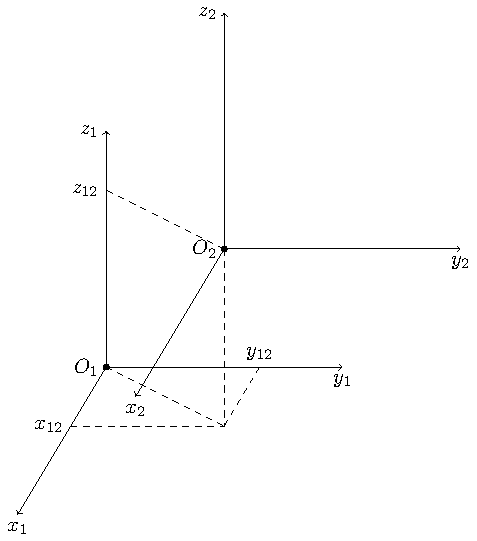
\includegraphics[width=8cm]{cartesian.pdf}
%\caption{Декартовые системы координат, произвольно сдвинутые друг относительно друга}
%\end{figure}
Связь между различными криволинейными координатами определяется формулами:
\begin{equation*}
{x_i} = {\rho _i}\cos {\varphi _i} = {r_i}\sin {\theta _i}\cos {\varphi _i} = {c_i}{\mathop{\rm sh}\nolimits} {\xi _i}\sin {\eta _i}\cos {\varphi _i} = {\tilde c_i}{\mathop{\rm ch}\nolimits} {\tilde \xi _i}\sin {\tilde \eta _i}\cos {\varphi _i},
\end{equation*}
\begin{equation*}
{y_i} = {\rho _i}\sin {\varphi _i} = {r_i}\sin {\theta _i}\sin {\varphi _i} = {c_i}{\mathop{\rm sh}\nolimits} {\xi _i}\sin {\eta _i}\sin {\varphi _i} = {\tilde c_i}{\mathop{\rm ch}\nolimits} {\tilde \xi _i}\sin {\tilde \eta _i}\sin {\varphi _i},
\end{equation*}
\begin{equation}\label{eq:1:2}
{z_i} = {r_i}\cos {\theta _i} = {c_i}{\mathop{\rm ch}\nolimits} {\xi _i}\cos {\eta _i} = {\tilde c_i}{\mathop{\rm sh}\nolimits} {\tilde \xi _i}\cos {\tilde \eta _i},
\end{equation}
\noindent где ${x_i},{y_i},{z_i} \in \left( { - \infty ;\infty } \right)$; ${\rho _i},{r_i},{\xi _i} \in \left[ {\left. {0;\infty } \right)} \right.$; ${\eta _i} \in \left[ {0;\pi } \right]$; ${\tilde \xi _i} \in \left( { - \infty ,\infty } \right)$; ${\tilde \eta _i} \in \left[ {0;\dfrac{\pi }{2}} \right]$; $\varphi  \in \left[ {0;2\pi } \right]$; ${c_i},{\tilde c_i}$ $\left( {{c_i},{{\tilde c}_i} > 0} \right)$~--- параметры сфероидальных систем координат.

В дальнейшем понадобятся базисные решения уравнения Лапласа

\begin{equation}
\Delta u = 0,
\end{equation}
\noindent регулярные вне (знак ``+'' в верхнем индексе), внутри (знак ``--'' в верхнем индексе) цилиндра $\Omega _3^ \pm$, шара $\Omega _4^ \pm$, вытянутого $\Omega _5^ \pm $ и сжатого $\Omega _6^ \pm $ сфероидов:

\begin{equation}\label{eq:1:4}
u_{\lambda ,m}^{ \pm (3)}\left( {\rho ,z,\varphi } \right) = {e^{i\lambda z + im\varphi }}\left\{ \begin{array}{l}
{{\tilde K}_m}\left( {\lambda \rho } \right)\\
{I_m}\left( {\lambda \rho } \right)
\end{array} \right\},\qquad {\kern 1pt} \lambda  \in \mathbb{R},\quad m \in \mathbb{Z};
\end{equation}

\begin{equation}\label{eq:1:5}
u_{n,m}^{ \pm (4)}\left( {r,\theta ,\varphi } \right) = \left\{ \begin{array}{l}
(n - m)!/{r^{n + 1}}\\
{r^n}/(n + m)!
\end{array} \right\}P_n^m(\cos \theta ){e^{im\varphi }};
\end{equation}
$$
n,m \in \mathbb{Z}, n\ge 0, |m| \le n;
$$
\begin{equation}\label{eq:1:6}
u_{n,m}^{ \pm (5)}\left( {\xi ,\eta ,\varphi } \right) = \left\{ \begin{array}{l}
Q_n^{ - m}({\mathop{\rm ch}\nolimits} \xi )\\
P_n^{ - m}({\mathop{\rm ch}\nolimits} \xi )
\end{array} \right\}P_n^m(\cos \eta ){e^{im\varphi }};
\end{equation}
$$
n,m \in \mathbb{Z}, n\ge 0, |m| \le n;
$$
\begin{equation}\label{eq:1:7}
u_{n,m}^{ \pm (6)}\left( {\tilde \xi ,\tilde \eta ,\varphi } \right) = \left\{ \begin{array}{l}
Q_n^{ - m}(i{\mathop{\rm sh}\nolimits} \tilde \xi )\\
P_n^{ - m}(i{\mathop{\rm sh}\nolimits} \tilde \xi )
\end{array} \right\}P_n^m(\cos \tilde \eta ){e^{im\varphi }};
\end{equation}
$$
n,m \in \mathbb{Z}, n\ge 0, |m| \le n;
$$
\noindent где ${I_m}(x)$~--- модифицированная функция Бесселя, $${\tilde K_m}(x) = {({\rm{sign}}{\mkern 1mu} {\kern 1pt} x)^m}{K_m}\left( {|x|} \right),$$
${K_m}(x)$~--- функция Макдональда, $P_n^m(x)$, $Q_n^m(x)$~--- функции Лежандра первого и второго рода. Верхний (нижний) множитель в фигурных скобках соответствует верхнему (нижнему) знаку индекса $\left\{  \pm  \right\}$.

В дальнейшем важную роль играют теоремы сложения решений~\eqref{eq:1:4}~-- \eqref{eq:1:7} в парах однотипных систем координат, описанных выше.

\begin{theorem}
При ${\rho _2} < {\rho _{12}}$ справедливо разложение
\begin{equation}\label{eq:1:8}
u_{\lambda ,m}^{ + (3)}\left( {{\rho _1},{z_1},{\varphi _1}} \right) = \sum\limits_{l =  - \infty }^\infty  {{{( - 1)}^l}} u_{m - l,\lambda }^{ + (3)}\left( {{\rho _{12}},{z_{12}},{\varphi _{12}}} \right)u_{l,\lambda }^{ - (3)}\left( {{\rho _2},{z_2},{\varphi _2}} \right).
\end{equation}

При ${\rho _1} < {\rho _{12}}$ справедливо разложение
\begin{equation}\label{eq:1:9}
u_{\lambda ,m}^{ + (3)}\left( {{\rho _2},{z_2},{\varphi _2}} \right) = \sum\limits_{l =  - \infty }^\infty  {{{( - 1)}^m}} u_{m - l,\lambda }^{ + (3)}\left( {{\rho _{12}}, - {z_{12}},{\varphi _{12}}} \right)u_{l,\lambda }^{ - (3)}\left( {{\rho _1},{z_1},{\varphi _1}} \right).
\end{equation}
\end{theorem}
%\begin{proof}
%Рассмотрим интегральное представление функции~\cite{Nikolaev1998-1}
%
%\begin{equation}\label{eq:1:10}
%u_{\lambda ,m}^{ + (3)}\left( {{\rho _1},{z_1},{\varphi _1}} \right) = {({\rm{sign}}{\mkern 1mu} {\kern 1pt} \lambda )^m}\frac{1}{2}\int\limits_{ - \infty }^\infty  {{e^{|\lambda |\left[ {i{z_1} - {\rho _1}{\mathop{\rm ch}\nolimits} (t - i{\varphi _1})} \right] + mt}}} dt,
%\end{equation}
%
%$\lambda  \ne 0$, ${\rho _1} > 0$, ${\varphi _1} \in \left( { - \dfrac{\pi }{2};\dfrac{\pi }{2}} \right)$. С учетом формул~\eqref{eq:1:1} запишем
%\begin{multline}\label{eq:1:11}
%i{z_1} - {\rho _1}{\mathop{\rm ch}\nolimits} (t - i{\varphi _1}) = i{z_1} - {\rho _1}\cos ({\varphi _1} + it) = i{z_1} - {\rho _1}\cos {\varphi _1}{\mathop{\rm ch}\nolimits} t - \\
%- i{\rho _1}\sin {\varphi _1}{\mathop{\rm sh}\nolimits} t = i{z_1} - {x_1}{\mathop{\rm ch}\nolimits} t - i{y_1}{\mathop{\rm sh}\nolimits} t = i{z_2} - {x_2}{\mathop{\rm ch}\nolimits} t - i{y_2}{\mathop{\rm sh}\nolimits} t + \\
%+ i{z_{12}} - {x_{12}}{\mathop{\rm ch}\nolimits} t - i{y_{12}}{\mathop{\rm sh}\nolimits} t = \\
%= i{z_2} - {\rho _2}{\mathop{\rm ch}\nolimits} (t - i{\varphi _2}) + i{z_{12}} - {\rho _{12}}{\mathop{\rm ch}\nolimits} (t - i{\varphi _{12}}).
%\end{multline}
%
%Подставим выражение~\eqref{eq:1:11}в интегральное представление~\eqref{eq:1:10} и преобразуем один из подынтегральных множителей ${e^{ - |\lambda |{\rho _2}{\mathop{\rm ch}\nolimits} (t - i{\varphi _2})}}$. Для этого воспользуемся производящей функцией для функции Бесселя~\cite{Lebedev}
%
%\begin{equation}
%{e^{\frac{u}{2}\left( {s - \frac{1}{s}} \right)}} = \sum\limits_{l =  - \infty }^\infty  {{s^l}} {J_l}(u).
%\end{equation}
%
%Подставим в тождество~\eqref{eq:1:2} $s = i{e^{t - i{\varphi _2}}}$, $u = i|\lambda |{\rho _2}$. В результате получим
%
%\begin{equation}\nonumber
%{e^{ - |\lambda |{\rho _2}{\mathop{\rm ch}\nolimits} \left( {t - i{\varphi _2}} \right)}} = \sum\limits_{l =  - \infty }^\infty  {{i^l}} {e^{tl - il{\varphi _2}}}{i^l}{I_l}\left( {|\lambda |{\rho _2}} \right).
%\end{equation}
%
%После замены индекса суммирования $l$ на $-l$ в последней формуле имеем разложение
%
%\begin{equation}\label{eq:1:13}
%{e^{ - |\lambda |{\rho _2}{\mathop{\rm ch}\nolimits} \left( {t - i{\varphi _2}} \right)}} = \sum\limits_{l =  - \infty }^\infty  {{{( - 1)}^l}} {e^{ - tl + il{\varphi _2}}}{I_l}\left( {|\lambda |{\rho _2}} \right).
%\end{equation}
%
%Подстановка~\eqref{eq:1:11} и~\eqref{eq:1:13} в~\eqref{eq:1:10} приводит к следующей цепочке равенств:
%
%\[u_{\lambda ,m}^{ + (3)}\left( {{\rho _1},{z_1},{\varphi _1}} \right) = {({\rm{sign}}{\mkern 1mu} {\kern 1pt} \lambda )^m}\frac{1}{2}\int\limits_{ - \infty }^\infty  {{e^{i\lambda {z_{12}} - |\lambda |{\rho _{12}}{\mathop{\rm ch}\nolimits} \left( {t - i{\varphi _{12}}} \right) + mt}}}  \times \]
%\[ \times \sum\limits_{l =  - \infty }^\infty  {{{( - 1)}^l}} {e^{ - tl + il{\varphi _2} + i\lambda {z_2}}}{I_l}\left( {|\lambda |{\rho _2}} \right) = \sum\limits_{l =  - \infty }^\infty  {{{( - 1)}^l}} u_{\lambda ,l}^{ - (3)}\left( {{\rho _2},{z_2},{\varphi _2}} \right) \times \]
%\[ \times {\left( {{\rm{sign}}{\mkern 1mu} {\kern 1pt} \lambda } \right)^{m - l}}\frac{1}{2}\int\limits_{ - \infty }^\infty  {{e^{i\lambda {z_{12}} - |\lambda |{\rho _{12}}{\mathop{\rm ch}\nolimits} \left( {t - i{\varphi _{12}}} \right) + (m - l)t}}} dt = \]
%\begin{equation}
%= \sum\limits_{l =  - \infty }^\infty  {u_{\lambda ,m - l}^{ + (3)}} \left( {{\rho _{12}},{z_{12}},{\varphi _{12}}} \right)u_{\lambda ,l}^{ - (3)}\left( {{\rho _2},{z_2},{\varphi _2}} \right).
%\end{equation}
%
%Разложение~\eqref{eq:1:9} доказывается аналогично.
%\end{proof}

\begin{theorem}
При ${r_2} < {r_{12}}$ справедливо разложение
\begin{equation}\label{eq:1:15}
u_{n,m}^{ + (4)}\left( {{r_1},{\theta _1},{\varphi _1}} \right) = \sum\limits_{k = 0}^\infty  {\sum\limits_{l =  - k}^k {{{( - 1)}^{k + l}}} } u_{n + k,m - l}^{ + (4)}\left( {{r_{12}},{\theta _{12}},{\varphi _{12}}} \right)u_{k,l}^{ - (4)}\left( {{r_2},{\theta _2},{\varphi _2}} \right).
\end{equation}
При  ${r_1} < {r_{12}}$
\begin{equation}
u_{n,m}^{ + (4)}\left( {{r_2},{\theta _2},{\varphi _2}} \right) = \sum\limits_{k = 0}^\infty  {\sum\limits_{l =  - k}^k {{{( - 1)}^{n + l}}} } u_{n + k,m - l}^{ + (4)}\left( {{r_{12}},{\theta _{12}},{\varphi _{12}}} \right)u_{k,l}^{ - (4)}\left( {{r_1},{\theta _1},{\varphi _1}} \right).
\label{eq:1:16a}
\end{equation}
\end{theorem}
%\begin{proof}
%Рассмотрим интегральное представление функции~\cite{Nikolaev1998-1}
%
%\[u_{n,m}^{ + (4)}\left( {{r_1},{\theta _1},{\varphi _1}} \right) = \frac{{n!}}{{2\pi i}}\int\limits_{ - \infty }^\infty  {{e^{mt}}} \left\{ {\frac{{{e^{i\frac{{\pi m}}{2}}}}}{{{{\left[ {{z_1} - i{\rho _1}{\mathop{\rm ch}\nolimits} \left( {t - i{\varphi _1}} \right)} \right]}^{n + 1}}}} - } \right.\]
%\begin{equation}\label{eq:1:17}
%- \left. {\frac{{{e^{ - i\frac{{\pi m}}{2}}}}}{{{{\left[ {{z_1} + i{\rho _1}{\mathop{\rm ch}\nolimits} \left( {t - i{\varphi _1}} \right)} \right]}^{n + 1}}}}} \right\}dt,
%\end{equation}
%\[{r_1} > 0,\quad {\theta _1} \in (0;\pi ),\quad {\varphi _1} \in \left( { - \frac{\pi }{2};\frac{\pi }{2}} \right),\quad n \ge |m|.\]
%
%Аналогично равенству~\eqref{eq:1:11} получаем
%
%\begin{multline}\label{eq:1:18}
%{z_1} \pm i{\rho _1}{\mathop{\rm ch}\nolimits} \left( {t - i{\varphi _1}} \right) = \\
%= {z_2} \pm i{\rho _2}{\mathop{\rm ch}\nolimits} \left( {t - i{\varphi _2}} \right) + {z_{12}} \pm i{\rho _{12}}{\mathop{\rm ch}\nolimits} \left( {t - i{\varphi _{12}}} \right).
%\end{multline}
%
%Разложим функцию ${\left[ {{z_1} \pm i{\rho _1}{\mathop{\rm ch}\nolimits} \left( {t - i{\varphi _1}} \right)} \right]^{ - n - 1}}$ в степенной ряд по степеням ${z_2} \pm i{\rho _2}{\mathop{\rm ch}\nolimits} \left( {t - i{\varphi _2}} \right)$:
%
%\begin{multline}\label{eq:1:19}
%{\left[ {{z_1} \pm i{\rho _1}{\mathop{\rm ch}\nolimits} \left( {t - i{\varphi _1}} \right)} \right]^{ - n - 1}} = \\
%= \sum\limits_{k = 0}^\infty  {{{( - 1)}^k}} \frac{{(n + k)!}}{{n!k!}}\frac{{{{\left[ {{z_2} \pm i{\rho _2}{\mathop{\rm ch}\nolimits} \left( {t - i{\varphi _2}} \right)} \right]}^k}}}{{{{\left[ {{z_{12}} \pm i{\rho _{12}}{\mathop{\rm ch}\nolimits} \left( {t - i{\varphi _{12}}} \right)} \right]}^{n + k + 1}}}}.
%\end{multline}
%
%Разложение сходится при условии
%
%\[|{z_2} \pm i{\rho _2}{\mathop{\rm ch}\nolimits} \left( {t - i{\varphi _2}} \right)| < |{z_{12}} \pm i{\rho _{12}}{\mathop{\rm ch}\nolimits} \left( {t - i{\varphi _{12}}} \right)|.\]
%
%Ряд~\eqref{eq:1:9} подставим в интегральное представление~\eqref{eq:1:17}. В результате получаем
%
%\begin{multline}\label{eq:1:20}
%u_{n,m}^{ + (4)}\left( {{r_1},{\theta _1},{\varphi _1}} \right) = \frac{{n!}}{{2\pi i}}\mathop \sum \limits_{k = 0}^\infty  {( - 1)^k}\frac{{(n + k)!}}{{n!k!}}\times\\
%\times\int\limits_{ - \infty }^\infty  {{e^{mt}}} \left\{ {\frac{{{{\left[ {{z_2} \pm i{\rho _2}{\mathop{\rm ch}\nolimits} \left( {t - i{\varphi _2}} \right)} \right]}^k}}}{{{{\left[ {{z_{12}} \pm i{\rho _{12}}{\mathop{\rm ch}\nolimits} \left( {t - i{\varphi _{12}}} \right)} \right]}^{n + k + 1}}}} - } \right.\\
%\left. { - {e^{ - i\frac{{\pi m}}{2}}}\frac{{{{\left[ {{z_2} \pm i{\rho _2}{\mathop{\rm ch}\nolimits} \left( {t - i{\varphi _2}} \right)} \right]}^k}}}{{{{\left[ {{z_{12}} \pm i{\rho _{12}}{\mathop{\rm ch}\nolimits} \left( {t - i{\varphi _{12}}} \right)} \right]}^{n + k + 1}}}}} \right\}dt.
%\end{multline}
%
%Запишем функцию ${\left[ {{z_2} \pm i{\rho _2}{\mathop{\rm ch}\nolimits} \left( {t - i{\varphi _2}} \right)} \right]^k}$ рядом Фурье по угловой координате~\cite{Lebedev}:
%
%\begin{multline}\label{eq:1:21}
%{\left[ {{z_2} \pm i{\rho _2}{\mathop{\rm ch}\nolimits} \left( {t - i{\varphi _2}} \right)} \right]^k} = r_2^k{\left[ {\cos {\theta _2} \pm i\sin {\theta _2}\cos \left( {{\varphi _2} + it} \right)} \right]^k} = \\
%= r_2^k\sum\limits_{l =  - k}^k {\frac{{k!}}{{(k + l)!}}} {e^{ \mp i\frac{{\pi l}}{2}}}P_k^l\left( {\cos {\theta _2}} \right){e^{il{\varphi _2} - lt}}.
%\end{multline}
%
%Подстановка~\eqref{eq:1:21} в формулу~\eqref{eq:1:20} приводит к следующему равенству:
%
%\begin{multline*}
%u_{n,m}^{ + (4)}\left( {{r_1},{\theta _1},{\varphi _1}} \right) = \sum\limits_{k = 0}^\infty  {{{( - 1)}^k}} (n + k)!\sum\limits_{l =  - \infty }^\infty  {\frac{1}{{(k + l)!}}} r_2^kP_k^l\left( {\cos {\theta _2}} \right){e^{il{\varphi _2}}} \times \\
%\times \frac{1}{{2\pi i}}\int\limits_{ - \infty }^\infty  {{e^{(m - l)t}}} \bigg\{ \frac{{{e^{i\frac{\pi }{2}(m + l)}}}}{{{{\left[ {{z_{12}} - i{\rho _{12}}{\mathop{\rm ch}\nolimits} \left( {t - i{\varphi _{12}}} \right)} \right]}^{n + k + 1}}}} - \\
%- \frac{{{e^{ - i\frac{\pi }{2}(m + l)}}}}{{{{\left[ {{z_{12}} + i{\rho _{12}}{\mathop{\rm ch}\nolimits} \left( {t - i{\varphi _{12}}} \right)} \right]}^{n + k + 1}}}} \bigg\}dt.
%\end{multline*}
%
%В силу интегрального представления~\eqref{eq:1:17}
%
%\begin{multline*}
%\frac{{(n + k)!}}{{2\pi i}}\int\limits_{ - \infty }^\infty  {{e^{(m - l)t}}} \left\{ \frac{{{e^{i\frac{\pi }{2}(m + l)}}}}{{{{\left[ {{z_{12}} - i{\rho _{12}}{\mathop{\rm ch}\nolimits} \left( {t - i{\varphi _{12}}} \right)} \right]}^{n + k + 1}}}} - \right.\\
%\left. - \frac{{{e^{ - i\frac{\pi }{2}(m + l)}}}}{{{{\left[ {{z_{12}} + i{\rho _{12}}{\mathop{\rm ch}\nolimits} \left( {t - i{\varphi _{12}}} \right)} \right]}^{n + k + 1}}}} \right\}dt =
%{e^{i\pi l}}u_{n + k,m - l}^{ + (4)}\left( {{r_{12}},{\theta _{12}},{\varphi _{12}}} \right).
%\end{multline*}
%
%Таким образом, получаем следующее разложение базисного решения уравнения Лапласа:
%
%\[u_{n,m}^{ + (4)}\left( {{r_1},{\theta _1},{\varphi _1}} \right) = \sum\limits_{k = 0}^\infty  {{{( - 1)}^{k + l}}} u_{n + k,m - l}^{ + (4)}\left( {{r_{12}},{\theta _{12}},{\varphi _{12}}} \right)u_{k,l}^{ - (4)}\left( {{r_2},{\theta _2},{\varphi _2}} \right).\]
%
%Теорема сложения~\eqref{eq:1:16a} получается аналогично.
%\end{proof}

\begin{theorem}
При ${\xi _2} \in \left( {0;{\gamma _2}} \right)$ справедливо разложение
\begin{multline}\label{eq:1:22}
u_{n,m}^{ + (5)}\left( {{\xi _1},{\eta _1},{\varphi _1}} \right) = \sum\limits_{s = 0}^\infty  {\sum\limits_{l =  - \infty }^\infty  {{{( - 1)}^{l + m}}} } u_{s,l}^{ - (5)}\left( {{\xi _2},{\eta _2},{\varphi _2}} \right) \times \\
\times \sum\limits_{q = 0}^\infty  {\frac{{\sqrt \pi  }}{{q!\Gamma \left( {n + q + \frac{3}{2}} \right)}}} {\left( {\frac{{{c_1}}}{2}} \right)^{2q + n + 1}}\sum\limits_{k = s}^\infty  {{{( - 1)}^k}} g_{k,l}^{ - (45)s}({c_2}) u_{2q + n + k,m - l}^{ + (4)}\left( {{r_{12}},{\theta _{12}},{\varphi _{12}}} \right).
\end{multline}

При ${\xi _1} \in \left( {0;{\gamma _1}} \right)$ справедливо разложение
\begin{multline}\label{eq:1:23}
u_{n,m}^{ + (5)}\left( {{\xi _2},{\eta _2},{\varphi _2}} \right) = \sum\limits_{s = 0}^\infty  {\sum\limits_{l =  - \infty }^\infty  {{{( - 1)}^{l + m}}} } u_{s,l}^{ - (5)}\left( {{\xi _1},{\eta _1},{\varphi _1}} \right) \times \\
\times \sum\limits_{q = 0}^\infty  {\frac{{\sqrt \pi  }}{{q!\Gamma \left( {n + q + \frac{3}{2}} \right)}}} {\left( {\frac{{{c_2}}}{2}} \right)^{2q + n + 1}}\sum\limits_{k = s}^\infty  {{{( - 1)}^n}} g_{k,l}^{ - (45)s}({c_1}) u_{2q + n + k,m - l}^{ + (4)}\left( {{r_{12}},{\theta _{12}},{\varphi _{12}}} \right).
\end{multline}

Выше использованы обозначения
\begin{equation}\label{eq:1:24}
{\gamma _j} = {\rm{Arsh}}{\mkern 1mu} {\kern 1pt} {\left[ {\frac{{t^2_j + \rho _{12}^2 - c_j^2 + \sqrt {\left( {t^2_j + \rho _{12}^2 - c_j^2} \right)^2 + 4\rho _{12}^2c_j^2} }}{{2c_j^2}}} \right]^{\frac{1}{2}}},
\end{equation}
$t_j=\max(|z_{12}|-c_{3-j},0)$,
\begin{equation}\label{eq:1:25}
g_{k,l}^{ - (45)s}({c_j}) = \sqrt \pi  {\varepsilon _{ks}}{\left( {\dfrac{{{c_j}}}{2}} \right)^k}\dfrac{{s + \dfrac{1}{2}}}{{\Gamma \left( {\dfrac{k}{2} - \dfrac{s}{2} + 1} \right)\Gamma \left( {\dfrac{k}{2} + \dfrac{s}{2} + \dfrac{3}{2}} \right)}},
\end{equation}
\begin{equation}\label{eq:1:26}
\varepsilon_{ks}=\left\{ {\begin{array}{*{20}{l}}
{1,\quad k - s = 2p,\quad p \in \mathbb{Z},}\\
{0,\quad k - s = 2p + 1,\quad p \in \mathbb{Z}.}
\end{array}} \right.
\end{equation}
$\Gamma (x)$~--- гамма-функция Эйлера.
\end{theorem}

%\begin{proof}
%Рассмотрим интегральное представление~\cite{Nikolaev1998-1}:
%\begin{multline}\label{eq:1:27}
%u_{n,m}^{ + (5)}\left( {{\xi _1},{\eta _1},{\varphi _1}} \right) = \frac{{{i^{m + 1}}}}{{2\pi }}\int\limits_{ - \infty }^\infty  {{e^{mt}}} \left\{ {{Q_n}\left[ {\frac{{{z_1} + i{\rho _1}{\mathop{\rm ch}\nolimits} \left( {t - i{\varphi _1}} \right)}}{{{c_1}}}} \right] + } \right. \\
%\left. { + {{( - 1)}^{n + m}}{Q_n}\left[ {\frac{{ - {z_1} + i{\rho _1}{\mathop{\rm ch}\nolimits} \left( {t - i{\varphi _1}} \right)}}{{{c_1}}}} \right]} \right\}dt.
%\end{multline}
%
%Разложим функцию Лежандра второго рода в гипергеометрический ряд по степеням ее аргумента~\cite{Lebedev}:
%
%\begin{equation}\label{eq:1:28}
%{Q_n}(u) = \sqrt \pi  \sum\limits_{q = 0}^\infty  {\frac{{(n + 2q)!}}{{q!{\mkern 1mu} {\kern 1pt} \Gamma \left( {n + q + \frac{3}{2}} \right)}}} {\left( {\frac{1}{{2n}}} \right)^{2q + n + 1}}.
%\end{equation}
%
%В качестве аргумента в последней формуле выберем выражение $$\dfrac{{{z_1} \pm i{\rho _1}{\mathop{\rm ch}\nolimits} \left( {t - i{\varphi _1}} \right)}}{{{c_1}}},$$ которое представим формулой~\eqref{eq:1:19}. В результате получим
%
%\begin{multline}\label{eq:1:29}
%{Q_n}\left[ {\frac{{ \pm {z_1} + i{\rho _1}{\mathop{\rm ch}\nolimits} \left( {t - i{\varphi _1}} \right)}}{{{c_1}}}} \right] = \sqrt \pi  \sum\limits_{q = 0}^\infty  {\frac{{{{( \pm 1)}^{n + 1}}}}{{q!\Gamma \left( {n + q + \frac{3}{2}} \right)}}} {\left( {\frac{{{c_1}}}{2}} \right)^{2q + n + 1}} \times \\
%\times \sum\limits_{k = 0}^\infty  {{{( - 1)}^k}} \frac{{(2q + n + k)!}}{{k!}}\frac{{{{\left[ {{z_2} \pm i{\rho _2}{\mathop{\rm ch}\nolimits} \left( {t - i{\varphi _2}} \right)} \right]}^k}}}{{{{\left[ {{z_{12}} \pm i{\rho _{12}}{\mathop{\rm ch}\nolimits} \left( {t - i{\varphi _{12}}} \right)} \right]}^{2q + n + k + 1}}}}.
%\end{multline}
%
%Используем совместно формулу~\eqref{eq:1:21} и теорему сложения гармонических функций в сферических и вытянутых сфероидальных системах координат с общим началом~\cite{Nikolaev2011}:
%
%\begin{equation}\label{eq:1:30}
%u_{k,l}^{ - (4)}\left( {{r_2},{\theta _2},{\varphi _2}} \right) = \sum\limits_{s = 0}^k {g_{k,l}^{ - (45)s}} ({c_2})u_{s,l}^{ - (5)}\left( {{\xi _2},{\eta _2},{\varphi _2}} \right),
%\end{equation}
%где $g_{k,l}^{ - (45)s}({c_2})$ описано в~\eqref{eq:1:25}. При этом получаем разложение
%
%\begin{multline}\label{eq:1:31}
%\frac{{{{\left[ {{z_2} \pm i{\rho _2}{\mathop{\rm ch}\nolimits} \left( {t - i{\varphi _2}} \right)} \right]}^k}}}{{k!}} = \\
%= \sum\limits_{l =  - \infty }^\infty  {{{( \mp i)}^l}} {e^{ - lt}}\sum\limits_{s = 0}^k {g_{k,l}^{ - (45)s}} ({c_2})u_{s,l}^{ - (5)}\left( {{\xi _2},{\eta _2},{\varphi _2}} \right).
%\end{multline}
%
%Формулы~\eqref{eq:1:29} и~\eqref{eq:1:31} подставим в интегральное представление~\eqref{eq:1:27}
%
%\begin{multline}\label{eq:1:32}
%u_{n,m}^{ + (5)}\left( {{\xi _1},{\eta _1},{\varphi _1}} \right) = \frac{{{i^{m + 1}}}}{{2\pi }}\sqrt \pi  \sum\limits_{q = 0}^\infty  {\frac{1}{{q!\Gamma \left( {n + q + \frac{3}{2}} \right)}}} {\left( {\frac{{{c_1}}}{2}} \right)^{2q + n + 1}} \times \\
%\times \sum\limits_{k = 0}^\infty  {{{( - 1)}^k}} (2q + n + k)!\sum\limits_{s = 0}^\infty  {\sum\limits_{l =  - \infty }^\infty  {g_{k,l}^{ - (45)s}} } ({c_2})u_{s,l}^{ - (5)}\left( {{\xi _2},{\eta _2},{\varphi _2}} \right) \times \\
%\times \int\limits_{ - \infty }^\infty  {{e^{(m - l)t}}} \left\{ {\frac{{{{( - i)}^l}}}{{{{\left[ {{z_{12}} + i{\rho _{12}}{\mathop{\rm ch}\nolimits} \left( {t - i{\varphi _{12}}} \right)} \right]}^{2q + n + k + 1}}}} + } \right.\\
%\left. { + {{( - 1)}^{n + m}}{{( - 1)}^{n + 1}}\frac{{{i^l}}}{{{{\left[ {{z_{12}} - i{\rho _{12}}{\mathop{\rm ch}\nolimits} \left( {t - i{\varphi _{12}}} \right)} \right]}^{2q + n + k + 1}}}}} \right\}dt.
%\end{multline}
%
%Интеграл в последней формуле может быть записан так:
%
%\begin{multline*}
%{( - 1)^l}{i^m}\int\limits_{ - \infty }^\infty  {{e^{(m - l)t}}} \left\{ {\frac{{{{( - i)}^{m - l}}}}{{{{\left[ {{z_{12}} + i{\rho _{12}}{\mathop{\rm ch}\nolimits} \left( {t - i{\varphi _{12}}} \right)} \right]}^{2q + n + k + 1}}}} - } \right.\\
%\left. { - \frac{{{i^{m - l}}}}{{{{\left[ {{z_{12}} - i{\rho _{12}}{\mathop{\rm ch}\nolimits} \left( {t - i{\varphi _{12}}} \right)} \right]}^{2q + n + k + 1}}}}} \right\}dt.
%\end{multline*}
%
%Следовательно, в силу формулы~\eqref{eq:1:17} он равен
%
%\[\frac{{2\pi }}{{(2q + n + k)!}}{( - 1)^{l + 1}}{i^{m + 1}}u_{2q + n + k,m - l}^{ + (4)}\left( {{r_{12}},{\theta _{12}},{\varphi _{12}}} \right).\]
%
%Подстановка последнего выражения в формулу~\eqref{eq:1:32} и замена порядка суммирования доказывает разложение~\eqref{eq:1:22}. Теорема сложения~\eqref{eq:1:23} доказывается аналогично.
%\end{proof}

\begin{theorem}
При ${\tilde \xi _2} \in \left[ {0,{{\tilde \gamma }_2}} \right)$ справедливо разложение
\begin{multline}\label{eq:1:33}
u_{n,m}^{ + (6)}\left( {{{\tilde \xi }_1},{{\tilde \eta }_1},{\varphi _1}} \right) = \sum\limits_{s = 0}^\infty  {\sum\limits_{l =  - \infty }^\infty  {{{( - 1)}^{l + m}}} } u_{s,l}^{ - (6)}\left( {{{\tilde \xi }_2},{{\tilde \eta }_2},{\varphi _2}} \right) \times \\
\times \sqrt \pi  \sum\limits_{q = 0}^\infty  {\frac{{{{( - 1)}^q}{{( - i)}^{n + 1}}}}{{q!\Gamma \left( {n + q + \frac{3}{2}} \right)}}} {\left( {\frac{{{{\tilde c}_1}}}{2}} \right)^{2q + n + 1}} \times \\
\times \sum\limits_{k = s}^\infty  {{{( - 1)}^k}} g_{k,l}^{ - (46)s}({c_2})u_{2q + n + k,m - l}^{ + (4)}\left( {{r_{12}},{\theta _{12}},{\varphi _{12}}} \right).
\end{multline}
При ${\tilde \xi _1} \in \left[ {0,{{\tilde \gamma }_1}} \right)$ справедливо разложение
\begin{multline}\label{eq:1:34}
u_{n,m}^{ + (6)}\left( {{{\tilde \xi }_2},{{\tilde \eta }_2},{\varphi _2}} \right) = \sum\limits_{s = 0}^\infty  {\sum\limits_{l =  - \infty }^\infty  {{{( - 1)}^{l + m}}} } u_{s,l}^{ - (6)}\left( {{{\tilde \xi }_1},{{\tilde \eta }_1},{\varphi _1}} \right) \times \\
\times \sqrt \pi  \sum\limits_{q = 0}^\infty  {\frac{{{{( - 1)}^q}{{( - i)}^{n + 1}}}}{{q!\Gamma \left( {n + q + \frac{3}{2}} \right)}}} {\left( {\frac{{{{\tilde c}_2}}}{2}} \right)^{2q + n + 1}} \times \\
\times \sum\limits_{k = s}^\infty  {{{( - 1)}^n}} g_{k,l}^{ - (46)s}({c_1})u_{2q + n + k,m - l}^{ + (4)}\left( {{r_{12}},{\theta _{12}},{\varphi _{12}}} \right).
\end{multline}
Здесь использованы обозначения
\begin{equation}\label{eq:1:35}
{\tilde \gamma _j} = {\rm{Arsh}}{\mkern 1mu} {\kern 1pt} {\left[ {\frac{{z_{12}^2 + \rho _{12}^2 - \tilde c_j^2 + \sqrt {\left( {z_{12}^2 + \rho _{12}^2 - \tilde c_j^2} \right)^2 + 4z_{12}^2\tilde c_j^2} }}{{2\tilde c_j^2}}} \right]^{\frac{1}{2}}},
\end{equation}
\begin{equation}\label{eq:1:36}
g_{k,l}^{ - (46)s}({c_j}) = \sqrt \pi  {\varepsilon _{ks}}{( - i)^k}{\left( {\dfrac{{{{\tilde c}_j}}}{2}} \right)^k}\dfrac{{s + \dfrac{1}{2}}}{{\Gamma \left( {\dfrac{k}{2} - \dfrac{s}{2} + 1} \right)\Gamma \left( {\dfrac{k}{2} + \dfrac{s}{2} + \dfrac{3}{2}} \right)}},
\end{equation}
\end{theorem}
%\begin{proof}
%Вывод формул~\eqref{eq:1:33} и~\eqref{eq:1:34} основан на интегральном представлении~\cite{Nikolaev1998-1}
%\begin{multline}\label{eq:1:37}
%u_{n,m}^{ + (6)}\left( {{{\tilde \xi }_1},{{\tilde \eta }_1},{\varphi _1}} \right) = \frac{{{{( - i)}^{m + 1}}}}{{2\pi }}\int\limits_{ - \infty }^\infty  {{e^{mt}}} \left\{ {{Q_n}\left[ {\frac{{i{z_1} + {\rho _1}{\mathop{\rm ch}\nolimits} \left( {t - i{\varphi _1}} \right)}}{{{{\tilde c}_1}}}} \right] + } \right.\\
%\left. { + {{( - 1)}^{n + m}}{Q_n}\left[ {\frac{{ - i{z_1} + {\rho _1}{\mathop{\rm ch}\nolimits} \left( {t - i{\varphi _1}} \right)}}{{{{\tilde c}_1}}}} \right]} \right\}dt,
%\end{multline}
%
%\noindent ${\tilde \xi _1} > 0$, ${\tilde \eta _1} \in (0,\pi )$, ${x_1} > \tilde c$, $n \ge |m|$, $n,m\in\mathbb{Z}$. Он может быть произведен так же, как в теореме 1.1.3.
%\end{proof}

\section{Теоремы сложения базисных решений уравнения Ламе в~сфероидальных координатах}

Приведенные в предыдущем параграфе свойства гармонических функций играют существенную роль при моделировании на\-пря\-жен\-но-де\-фор\-ми\-ро\-ван\-но\-го состояния многосвязного упругого тела.

Будем рассматривать однородную изотропную упругую среду. Вектор перемещений ${\bf{U}}$ точек среды, как известно, описывается уравнением Ламе

\begin{equation}\label{eq:1:38}
\Delta {\bf{U}} + \frac{1}{{1 - 2\sigma }}\nabla div{\bf{U}} = 0,
\end{equation}
\noindent где $\sigma$~--- коэффициент Пуассона; $\nabla$~--- оператор ``набла''.

В работах~\cite{Nikolaev1993,Nikolaev1984} были введены следующие частные решения уравнения~\eqref{eq:1:38} во внешности (внутренности) вытянутого сфероида $\Omega _5^ \pm = \Big\{ {(\xi ,\eta ,\varphi ): \- {\mkern 1mu} {\kern 1pt} \xi  \mathbin{\lower.3ex\hbox{$\buildrel>\over
{\smash{\scriptstyle<}\vphantom{_x}}$}} {\xi _0}} \Big\}$:

\begin{equation}\label{eq:1:39}
{\bf{U}}_{s,n,m}^{ \pm (5)}\left( {\xi ,\eta ,\varphi } \right) = \frac{c}{{2n + 1}}{{\bf{D}}_s}\left[ {u_{n - 1,m}^{ \pm (5)}\left( {\xi ,\eta ,\varphi } \right) - u_{n + 1,m}^{ \pm (5)}\left( {\xi ,\eta ,\varphi } \right)} \right];\,{\kern 1pt} s = 1,3;
\end{equation}

\begin{equation}\label{eq:1:40}
{\bf{U}}_{2,n,m}^{ \pm (5)}\left( {\xi ,\eta ,\varphi } \right) = {{\bf{D}}_2}u_{n,m}^{ \pm (5)}\left( {\xi ,\eta ,\varphi } \right) - c{{\mathop{\rm ch}\nolimits} ^2}{\xi _0}{{\bf{D}}_1}u_{n \pm 1,m}^{ \pm (5)}\left( {\xi ,\eta ,\varphi } \right),
\end{equation}

\noindent где $n = 0,{\mkern 1mu} {\kern 1pt} 1,{\mkern 1mu} {\kern 1pt}  \ldots $; $|m| \le n + 1$; $u_{n,m}^{ \pm (5)}$ определены в~\eqref{eq:1:6};

\begin{equation*}
{{\bf{D}}_1} = \nabla  = {{\bf{e}}_x}\frac{\partial }{{\partial x}} + {{\bf{e}}_y}\frac{\partial }{{\partial y}} + {{\bf{e}}_z}\frac{\partial }{{\partial z}};
\end{equation*}
\begin{equation}\label{eq:1:41}
{{\bf{D}}_2} = z\nabla  - \chi {{\bf{e}}_z};\quad {{\bf{D}}_3} = i\left[ {\nabla  \times {{\bf{e}}_z}} \right];
\end{equation}

\noindent $\chi  = 3 - 4\sigma $, $\left\{ {{{\bf{e}}_x},{{\bf{e}}_y},{{\bf{e}}_z}} \right\}$~--- орты декартовой системы координат.

В развернутой координатной форме формулы~\eqref{eq:1:39}~-- \eqref{eq:1:40} имеют вид:

\begin{equation}\label{eq:1:42}
{\bf{U}}_{1,n,m}^{ \pm (5)} = u_{n,m - 1}^{ \pm (5)}{{\bf{e}}_{ - 1}} - u_{n,m + 1}^{ \pm (5)}{{\bf{e}}_1} - u_{n,m}^{ \pm (5)}{{\bf{e}}_0};
\end{equation}

\begin{multline}\label{eq:1:43}
{\bf{U}}_{2,n,m}^{ \pm (5)} = qu_{1,n,m - 1}^{ \pm (5)}{{\bf{e}}_{ - 1}} - qu_{1,n,m + 1}^{ \pm (5)}{{\bf{e}}_1} - \left[ {qu_{1,n,m}^{ \pm (5)} + \chi u_{n,m}^{ \pm (5)}} \right]{{\bf{e}}_0} + \\
+ c\left( {{q^2} - q_0^2} \right)\nabla u_{n \pm 1,m}^{ \pm (5)};
\end{multline}

\begin{equation}\label{eq:1:44}
{\bf{U}}_{3,n,m}^{ \pm (5)} =  - u_{n,m - 1}^{ \pm (5)}{{\bf{e}}_{ - 1}} - u_{n,m + 1}^{ \pm (5)}{{\bf{e}}_1}.
\end{equation}

Здесь использованы обозначения

\begin{equation*}
u_{1,n,m}^{ \pm (5)} = u_{1,n,m}^ \pm (\xi )P_n^m(\cos \eta ){e^{im\varphi }};\quad
u_{1,n,m}^ \pm (\xi ) = \left\{ \begin{array}{l}
(n + m + 1)Q_{n + 1}^{ - m}(q)\\
 - (n - m)P_{n - 1}^{ - m}(q)
\end{array} \right\};
\end{equation*}
\begin{equation}\label{eq:1:45}
q = {\mathop{\rm ch}\nolimits} \xi ,\quad {q_0} = {\mathop{\rm ch}\nolimits} {\xi _0},\quad {{\bf{e}}_{ \mp 1}} = \frac{1}{2}\left( {{{\bf{e}}_x} \pm i{{\bf{e}}_y}} \right),\quad {{\bf{e}}_0} = {{\bf{e}}_z}.
\end{equation}

В работе~\cite{Nikolaev1998} введено понятие базисности системы решений уравнения Ламе в односвязной канонической области и доказана базисность решений~\eqref{eq:1:39}~-- \eqref{eq:1:41} в соответствующих областях $\Omega _5^ \pm $.{\sloppy\par}

В дальнейшем нам понадобятся теоремы сложения базисных решений уравнения Ламе в одинаково направленных вытянутых сфероидальных системах координат, начала которых сдвинуты согласно соотношениям~\eqref{eq:1:1}.

\begin{theorem}
При ${\xi _2},{\mkern 1mu} {\kern 1pt} {\xi _{20}} \in (0;{\mkern 1mu} {\kern 1pt} {\gamma _2})$ справедливы разложения

\begin{equation}\label{eq:1:46}
{\bf{U}}_{s,n,m}^{ + (5)}\left( {{\xi _1},{\eta _1},{\varphi _1}} \right) = \sum\limits_{k = 0}^\infty  {\sum\limits_{l =  - \infty }^\infty  {f_{n,m}^{ + (55)k,l}} } {\bf{U}}_{s,k,l}^{ - (5)}\left( {{\xi _2},{\eta _2},{\varphi _2}} \right), {\kern 1pt} s = 1,{\mkern 1mu} {\kern 1pt} 3;
\end{equation}

\begin{multline}\label{eq:1:47}
{\bf{U}}_{2,n,m}^{ + (5)}\left( {{\xi _1},{\eta _1},{\varphi _1}} \right) = \sum\limits_{k = 0}^\infty  {\sum\limits_{l =  - \infty }^\infty  {\left[ {f_{n,m}^{ + (55)k,l}} \right.} } {\bf{U}}_{2,k,l}^{ - (5)}\left( {{\xi _2},{\eta _2},{\varphi _2}} \right) + \\
\left. { + \tilde f_{n,m}^{ + (55)k,l}{\bf{U}}_{1,k,l}^{ - (5)}\left( {{\xi _2},{\eta _2},{\varphi _2}} \right)} \right],
\end{multline}

\noindent где

\begin{equation}\label{eq:1:48}
f_{n,m}^{ + (55)k,l} = \sum\limits_{j = n}^\infty  {g_{n,m}^{ + (54)j}} ({c_1})f_{j,m}^{(45)k,l}({c_2});
\end{equation}

\begin{equation}\label{eq:1:49}
g_{n,m}^{ + (54)j}({c_1}) = {( - 1)^m}\sqrt \pi  {\left( {\frac{{{c_1}}}{2}} \right)^{j + 1}}\frac{{{\varepsilon _{jn}}}}{{\Gamma \left( {\frac{{j - n}}{2} + 1} \right)\Gamma \left( {\frac{{j + n}}{2} + \frac{3}{2}} \right)}};
\end{equation}

\begin{equation}\label{eq:1:50}
f_{j,m}^{(45)k,l}({c_2}) = \sum\limits_{p = 0}^\infty  {{{( - 1)}^{p + l}}} \sqrt \pi  {\left( {\frac{{{c_2}}}{2}} \right)^p}\frac{{{\varepsilon _{pk}}\left( {k + \frac{1}{2}} \right)u_{j + p,m - l}^{ + (4)}\left( {{r_{12}},{\theta _{12}},{\varphi _{12}}} \right)}}{{\Gamma \left( {\frac{{p - k}}{2} + 1} \right)\Gamma \left( {\frac{{p + k}}{2} + \frac{3}{2}} \right)}};
\end{equation}

\begin{multline}\label{eq:1:51}
\tilde f_{n,m}^{ + (55)k,l} = \sum\limits_{j = n}^\infty \bigg[ {c_2}q_{20}^2\frac{{2k + 1}}{{2k + 3}}g_{n,m}^{ + (54)j}({c_1})f_{j + 1,m}^{(45)k + 1,l}({c_2}) + \\
+ {z_{12}}g_{n,m}^{ + (54)j}({c_1})f_{j + 1,m}^{(45)k,l}({c_2}) - {{c_1}q_{10}^2g_{n + 1,m}^{ + (54)j - 1}({c_1})f_{j,m}^{(45)k,l}({c_2})} \bigg].
\end{multline}

При ${\xi _1},{\mkern 1mu} {\kern 1pt} {\xi _{10}} \in (0;{\mkern 1mu} {\kern 1pt} {\gamma _1})$ справедливы разложения

\begin{equation}\label{eq:1:52}
{\bf{U}}_{s,n,m}^{ + (5)}\left( {{\xi _2},{\eta _2},{\varphi _2}} \right) = \sum\limits_{k = 0}^\infty  {\sum\limits_{l =  - \infty }^\infty  {f_{n,m}^{ - (55)k,l}} } {\bf{U}}_{s,k,l}^{ - (5)}\left( {{\xi _1},{\eta _1},{\varphi _1}} \right), {\kern 1pt} s = 1,{\mkern 1mu} {\kern 1pt} 3;
\end{equation}

\begin{multline}\label{eq:1:53}
{\bf{U}}_{2,n,m}^{ + (5)}\left( {{\xi _2},{\eta _2},{\varphi _2}} \right) = \sum\limits_{k = 0}^\infty  {\sum\limits_{l =  - \infty }^\infty  {\left[ {f_{n,m}^{ - (55)k,l}} \right.} } {\bf{U}}_{2,k,l}^{ - (5)}\left( {{\xi _1},{\eta _1},{\varphi _1}} \right) + \\
\left. { + \tilde f_{n,m}^{ - (55)k,l}{\bf{U}}_{1,k,l}^{ - (5)}\left( {{\xi _1},{\eta _1},{\varphi _1}} \right)} \right],
\end{multline}

\noindent где

\begin{equation}\label{eq:1:54}
f_{n,m}^{ - (55)k,l} = \sum\limits_{j = k}^\infty  {f_{n,m}^{(54)j,l}({c_2})g_{j,l}^{ - (45)k}} ({c_1});
\end{equation}

\begin{equation}\label{eq:1:55}
f_{n,m}^{(54)j,l}({c_2}) = \sum\limits_{p = 0}^\infty  {{{( - 1)}^{p + l + m}}} \sqrt \pi  {\left( {\frac{{{c_2}}}{2}} \right)^{p + 1}}\frac{{{\varepsilon _{pn}}u_{p + j,m - l}^{ + (4)}\left( {{r_{12}},{\theta _{12}},{\varphi _{12}}} \right)}}{{\Gamma \left( {\frac{{p - n}}{2} + 1} \right)\Gamma \left( {\frac{{p + n}}{2} + \frac{3}{2}} \right)}};
\end{equation}

\begin{multline}\label{eq:1:56}
\tilde f_{n,m}^{ - (55)k,l} = \sum\limits_{j = k}^\infty  \bigg[ {c_2}q_{20}^2f_{n + 1,m}^{(54)j + 1,l}({c_2})g_{j,l}^{ - (45)k}({c_1}) + {z_{12}}f_{n,m}^{(54)j + 1,l}({c_2})g_{j,l}^{ - (45)k}({c_1}) - \\
- {c_1}q_{10}^2\frac{{2k + 1}}{{2k + 3}}f_{n,m}^{(54)j,l}({c_2})g_{j - 1,l}^{ - (45)k + 1}({c_1}) \bigg],
\end{multline}

\noindent $g_{j,l}^{ - (45)k}({c_1})$ описано формулой~\eqref{eq:1:25}.
\end{theorem}
%\begin{proof}
%Теорему сложения~\eqref{eq:1:22} можно записать в виде
%\begin{equation}\label{eq:1:57}
%u_{n,m}^{ + (5)}\left( {{\xi _1},{\eta _1},{\varphi _1}} \right) = \sum\limits_{k = 0}^\infty  {\sum\limits_{l =  - \infty }^\infty  {f_{n,m}^{ + (55)k,l}} } u_{k,l}^{ - (5)}\left( {{\xi _2},{\eta _2},{\varphi _2}} \right).
%\end{equation}
%
%Используя формулу~\eqref{eq:1:57}, преобразуем выражение
%
%\begin{multline}\label{eq:1:58}
%u_{n - 1,m}^{ + (5)}\left( {{\xi _1},{\eta _1},{\varphi _1}} \right) - u_{n + 1,m}^{ + (5)}\left( {{\xi _1},{\eta _1},{\varphi _1}} \right) = \\
%= \sum\limits_{k = 0}^\infty  {\sum\limits_{l =  - \infty }^\infty  {\left[ {f_{n - 1,m}^{ + (55)k,l} - f_{n + 1,m}^{ + (55)k,l}} \right]} } u_{k,l}^{ - (5)}\left( {{\xi _2},{\eta _2},{\varphi _2}} \right).
%\end{multline}
%
%Заметим, что переходные коэффициенты теоремы сложения~\eqref{eq:1:57} подчиняются следующему рекуррентному соотношению:
%
%\begin{equation}\label{eq:1:59}
%f_{n - 1,m}^{ + (55)k,l} - f_{n + 1,m}^{ + (55)k,l} = \frac{{2n + 1}}{{{c_1}}}\frac{{{c_2}}}{2}\left[ {\frac{{f_{n,m}^{ + (55)k + 1,l}}}{{k + \frac{3}{2}}} - \frac{{f_{n,m}^{ + (55)k - 1,l}}}{{k - \frac{1}{2}}}} \right].
%\end{equation}
%
%Действительно, нетрудно проверить, что
%
%\begin{equation}\label{eq:1:60}
%g_{n - 1,m}^{ + (54)j}({c_1}) - g_{n + 1,m}^{ + (54)j}({c_1}) = \frac{{2n + 1}}{{{c_1}}}g_{n,m}^{ + (54)j + 1}({c_1}).
%\end{equation}
%
%Преобразуем разность
%
%\begin{multline}\label{eq:1:61}
%\frac{{f_{n,m}^{ + (55)k + 1,l}({c_2})}}{{k + \frac{3}{2}}} - \frac{{f_{n,m}^{ + (55)k - 1,l}({c_2})}}{{k - \frac{1}{2}}} = \sum\limits_{p = k + 1}^\infty  {{{( - 1)}^{p + l}}} \sqrt \pi  {\left( {\frac{{{c_2}}}{2}} \right)^p} \times \\
%\times \frac{{{\varepsilon _{p,k + 1}}u_{j + p,m - l}^{ + (4)}\left( {{r_{12}},{\theta _{12}},{\varphi _{12}}} \right)}}{{\Gamma \left( {\frac{p}{2} - \frac{k}{2} + \frac{1}{2}} \right)\Gamma \left( {\frac{p}{2} + \frac{k}{2} + 2} \right)}} - \sum\limits_{p = k - 1}^\infty  {{{( - 1)}^{p + l}}} \sqrt \pi  {\left( {\frac{{{c_2}}}{2}} \right)^p} \times \\
%\times \frac{{{\varepsilon _{p,k - 1}}u_{j + p,m - l}^{ + (4)}\left( {{r_{12}},{\theta _{12}},{\varphi _{12}}} \right)}}{{\Gamma \left( {\frac{p}{2} - \frac{k}{2} + \frac{3}{2}} \right)\Gamma \left( {\frac{p}{2} + \frac{k}{2} + 2} \right)}} = \sum\limits_{p = k - 1}^\infty  {{{( - 1)}^{p + l}}} \sqrt \pi  {\left( {\frac{{{c_2}}}{2}} \right)^p} \times \\
%\times \frac{{{\varepsilon _{p,k - 1}}u_{j + p,m - l}^{ + (4)}\left( {{r_{12}},{\theta _{12}},{\varphi _{12}}} \right)}}{{\Gamma \left( {\frac{p}{2} - \frac{k}{2} + \frac{3}{2}} \right)\Gamma \left( {\frac{p}{2} + \frac{k}{2} + 2} \right)}}\left( { - k - \frac{1}{2}} \right).
%\end{multline}
%
%После изменения индекса суммирования $p$ на $p-1$ получаем
%
%\begin{multline}\label{eq:1:62}
%\frac{{f_{n,m}^{ + (55)k + 1,l}({c_2})}}{{k + \frac{3}{2}}} - \frac{{f_{n,m}^{ + (55)k - 1,l}({c_2})}}{{k - \frac{1}{2}}} = \frac{2}{{{c_2}}}\sum\limits_{p = k}^\infty  {{{( - 1)}^{p + l}}} \sqrt \pi  {\left( {\frac{{{c_2}}}{2}} \right)^p} \times \\
%\times \frac{{{\varepsilon _{pk}}u_{j + p - 1,m - l}^{ + (4)}\left( {{r_{12}},{\theta _{12}},{\varphi _{12}}} \right)}}{{\Gamma \left( {\frac{p}{2} - \frac{k}{2} + 1} \right)\Gamma \left( {\frac{p}{2} + \frac{k}{2} + \frac{3}{2}} \right)}}\left( {k + \frac{1}{2}} \right) = \frac{2}{{{c_2}}}f_{j - 1,m}^{(45)k,l}({c_2}).
%\end{multline}
%
%Теперь преобразуем разность, стоящую в левой части равенства~\eqref{eq:1:59}:
%
%\begin{multline}\label{eq:1:63}
%f_{n - 1,m}^{ + (55)k,l} - f_{n + 1,m}^{ + (55)k,l} = \sum\limits_{j = n - 1}^\infty  {g_{n - 1,m}^{ + (54)j}} ({c_1})f_{j,m}^{(45)k,l}({c_2}) - \\
%- \sum\limits_{j = n + 1}^\infty  {g_{n + 1,m}^{ + (54)j}} ({c_1})f_{j,m}^{(45)k,l}({c_2}) = \sum\limits_{j = n - 1}^\infty  {\left[ {g_{n - 1,m}^{ + (54)j}({c_1}) - } \right.} \\
%\left. { - g_{n + 1,m}^{ + (54)j}({c_1})} \right]f_{j,m}^{(45)k,l}({c_2}).
%\end{multline}
%
%Воспользуемся формулой~\eqref{eq:1:60}, после чего изменим индекс суммирования $j$ в сумме~\eqref{eq:1:63} на $j-1$. В результате получаем
%
%\begin{multline*}
%f_{n - 1,m}^{ + (55)k,l} - f_{n + 1,m}^{ + (55)k,l} = \sum\limits_{j = n - 1}^\infty  {\frac{{2n + 1}}{{{c_1}}}} g_{n,m}^{ + (54)j + 1}({c_1})f_{j,m}^{(45)k,l}({c_2}) = \\
%= \sum\limits_{j = n}^\infty  {\frac{{2n + 1}}{{{c_1}}}} g_{n,m}^{ + (54)j}({c_1})f_{j - 1,m}^{(45)k,l}({c_2}).
%\end{multline*}
%
%Преобразуя последнее выражение с использованием формулы~\eqref{eq:1:62}, окончательно получаем равенство~\eqref{eq:1:59}. Теперь подставим~\eqref{eq:1:59} в~\eqref{eq:1:58}:
%
%\begin{multline}\label{eq:1:64}
%u_{n - 1}^{ + (5)}\left( {{\xi _1},{\eta _1},{\varphi _1}} \right) - u_{n + 1,m}^{ + (5)}\left( {{\xi _1},{\eta _1},{\varphi _1}} \right) = \frac{{2n + 1}}{{{c_1}}}\frac{{{c_2}}}{2} \times \\
%\times \sum\limits_{k = 0}^\infty  {\sum\limits_{l =  - \infty }^\infty  {\left[ {\frac{{f_{n,m}^{ + (55)k + 1,l}}}{{k + \frac{3}{2}}} - \frac{{f_{n,m}^{ + (55)k - 1,l}}}{{k - \frac{1}{2}}}} \right]} } u_{k,l}^{ - (5)}\left( {{\xi _2},{\eta _2},{\varphi _2}} \right) = \\
%= \frac{{2n + 1}}{{{c_1}}}\frac{{{c_2}}}{2}\sum\limits_{k = 0}^\infty  {\sum\limits_{l =  - \infty }^\infty  {\frac{{f_{n,m}^{ + (55)k + 1,l}}}{{k + \frac{3}{2}}}} } u_{k,l}^{ - (5)}\left( {{\xi _2},{\eta _2},{\varphi _2}} \right) - \frac{{2n + 1}}{{{c_1}}}\frac{{{c_2}}}{2} \times \\
%\times \sum\limits_{k = 0}^\infty  {\sum\limits_{l =  - \infty }^\infty  {\frac{{f_{n,m}^{ + (55)k - 1,l}}}{{k - \frac{1}{2}}}} } u_{k,l}^{ - (5)}\left( {{\xi _2},{\eta _2},{\varphi _2}} \right).
%\end{multline}
%
%Применим к обеим частям равенства~\eqref{eq:1:64} дифференциальный оператор ${{\bf{D}}_s}$. После изменения индекса суммирования в первом выражении $k$ на $k+1$, а во втором~--- $k$ на $k-1$ получаем
%
%\begin{multline*}
%\frac{{{c_1}}}{{2n + 1}}{{\bf{D}}_s}\left[ {u_{n - 1,m}^{ + (5)}\left( {{\xi _1},{\eta _1},{\varphi _1}} \right) - u_{n + 1,m}^{ + (5)}\left( {{\xi _1},{\eta _1},{\varphi _1}} \right)} \right] = \\
%= \sum\limits_{k = 0}^\infty  {\sum\limits_{l =  - \infty }^\infty  {f_{n,m}^{ + (55)k,l}} } \frac{{{c_2}}}{{2k + 1}}{{\bf{D}}_s}\left[ {u_{k - 1,l}^{ - (5)}\left( {{\xi _2},{\eta _2},{\varphi _2}} \right) - u_{k + 1,l}^{ - (5)}\left( {{\xi _2},{\eta _2},{\varphi _2}} \right)} \right],
%\end{multline*}
%
%\noindent что доказывает формулу~\eqref{eq:1:46}.
%
%Теперь докажем формулу~\eqref{eq:1:47}. Для этого применим дифференциальный оператор~\eqref{eq:1:40} к формуле~\eqref{eq:1:57}:
%
%\begin{multline}\label{eq:1:65}
%{\bf{U}}_{2,n,m}^{ + (5)}\left( {{\xi _1},{\eta _1},{\varphi _1}} \right) = \sum\limits_{k = 0}^\infty  {\sum\limits_{l =  - \infty }^\infty  {f_{n,m}^{ + (55)k,l}} } \left[ {{z_1}\nabla  - \chi {{\bf{e}}_z}} \right]u_{k,l}^{ - (5)}\left( {{\xi _2},{\eta _2},{\varphi _2}} \right) - \\
%- {c_1}q_{10}^2\sum\limits_{k = 0}^\infty  {\sum\limits_{l =  - \infty }^\infty  {f_{n + 1,m}^{ + (55)k,l}} } \nabla u_{k,l}^{ - (5)}\left( {{\xi _2},{\eta _2},{\varphi _2}} \right) = \\
%= \sum\limits_{k = 0}^\infty  {\sum\limits_{l =  - \infty }^\infty  {f_{n,m}^{ + (55)k,l}} } \bigg\{ \left[ {{z_2}\nabla  - \chi {{\bf{e}}_z}} \right]u_{k,l}^{ - (5)}\left( {{\xi _2},{\eta _2},{\varphi _2}} \right) - \\
%- {c_2}q_{20}^2\nabla u_{k - 1,l}^{ - (5)}\left( {{\xi _2},{\eta _2},{\varphi _2}} \right) \bigg\} + \\
%+ \sum\limits_{k = 0}^\infty  {\sum\limits_{l =  - \infty }^\infty  {f_{n,m}^{ + (55)k,l}} } \left[ {{z_{12}}\nabla u_{k,l}^{ - (5)}\left( {{\xi _2},{\eta _2},{\varphi _2}} \right) + {c_2}q_{20}^2\nabla u_{k - 1,l}^{ - (5)}\left( {{\xi _2},{\eta _2},{\varphi _2}} \right)} \right] - \\
%- {c_1}q_{10}^2\sum\limits_{k = 0}^\infty  {\sum\limits_{l =  - \infty }^\infty  {f_{n + 1,m}^{ + (55)k,l}} } \nabla u_{k,l}^{ - (5)}\left( {{\xi _2},{\eta _2},{\varphi _2}} \right).
%\end{multline}
%
%Преобразуем коэффициенты с помощью рекуррентного соотношения~\eqref{eq:1:62}:{\sloppy\par}
%
%\begin{equation}\label{eq:1:66}
%f_{n,m}^{ + (55)k,l} = \sum\limits_{j = n}^\infty  {g_{n,m}^{ + (54)j}} ({c_1})\frac{{{c_2}}}{2}\left[ {\frac{{f_{j + 1,m}^{(45)k + 1,l}({c_2})}}{{k + \frac{3}{2}}} - \frac{{f_{j + 1,m}^{(45)k - 1,l}({c_2})}}{{k - \frac{1}{2}}}} \right].
%\end{equation}
%
%С учетом последней формулы получаем
%
%\begin{multline}\label{eq:1:67}
%\sum\limits_{k = 0}^\infty  {\sum\limits_{l =  - \infty }^\infty  {f_{n,m}^{ + (55)k,l}} } {z_{12}}\nabla u_{k,l}^{ - (5)}\left( {{\xi _2},{\eta _2},{\varphi _2}} \right) = \sum\limits_{k = 0}^\infty  \sum\limits_{l =  - \infty }^\infty  \sum\limits_{j = n}^\infty  {g_{n,m}^{ + (54)j}} ({c_1})\frac{{{c_2}}}{2}\times \\
%\times \left[ {\frac{{f_{j + 1,m}^{(45)k + 1,l}({c_2})}}{{k + \frac{3}{2}}} - \frac{{f_{j + 1,m}^{(45)k - 1,l}({c_2})}}{{k - \frac{1}{2}}}} \right] \nabla u_{k,l}^{ - (5)}\left( {{\xi _2},{\eta _2},{\varphi _2}} \right) = \\
%= \sum\limits_{k = 0}^\infty  {\sum\limits_{l =  - \infty }^\infty  {\sum\limits_{j = n}^\infty  {g_{n,m}^{ + (54)j}} } } ({c_1})f_{j + 1,m}^{(45)k,l}({c_2})\frac{{{c_2}}}{{2k + 1}}\nabla u_{k - 1,l}^{ - (5)}\left( {{\xi _2},{\eta _2},{\varphi _2}} \right) - \\
%- \sum\limits_{k = 0}^\infty  {\sum\limits_{l =  - \infty }^\infty  {\sum\limits_{j = n}^\infty  {g_{n,m}^{ + (54)j}} } } ({c_1})f_{j + 1,m}^{(45)k,l}({c_2})\frac{{{c_2}}}{{2k + 1}}\nabla u_{k + 1,l}^{ - (5)}\left( {{\xi _2},{\eta _2},{\varphi _2}} \right).
%\end{multline}
%
%Аналогично могут быть преобразованы остальные слагаемые в~\eqref{eq:1:65}. Таким образом, доказано разложение~\eqref{eq:1:47}. Подобным образом доказываются разложения~\eqref{eq:1:52}, \eqref{eq:1:53}. При этом используются рекуррентные соотношения
%
%\begin{equation}\label{eq:1:68}
%f_{n - 1,m}^{(54)j,l}({c_2}) - f_{n + 1,m}^{(54)j,l}({c_2}) =  - \frac{{2n + 1}}{{{c_2}}}f_{n,m}^{(54)j - 1,l}({c_2}),
%\end{equation}
%
%\begin{equation}\label{eq:1:69}
%\frac{{g_{j,l}^{ - (45)k - 1}({c_1})}}{{k - \frac{1}{2}}} - \frac{{g_{j,l}^{ - (45)k + 1}({c_1})}}{{k + \frac{3}{2}}} = \frac{2}{{{c_1}}}g_{j + 1,l}^{ - (45)k}({c_1}),
%\end{equation}
%
%\begin{equation}\label{eq:1:70}
%f_{n - 1,m}^{ - (55)k,l} - f_{n + 1,m}^{ - (55)k,l} =  - \frac{{2n + 1}}{{{c_2}}}\frac{{{c_1}}}{2}\left[ {\frac{{f_{n,m}^{ - (55)k - 1,l}}}{{k - \frac{1}{2}}} - \frac{{f_{n,m}^{ - (55)k + 1,l}}}{{k + \frac{3}{2}}}} \right].
%\end{equation}
%
%\end{proof}

Теперь рассмотрим частные решения уравнения Ламе для сжатого сфероида $\Omega _6^ \pm = \Big\{ {(\tilde \xi ,\tilde \eta ,\varphi ):{\mkern 1mu} {\mkern 1mu} {\kern 1pt} \tilde \xi  \mathbin{\lower.3ex\hbox{$\buildrel>\over
{\smash{\scriptstyle<}\vphantom{_x}}$}} {{\tilde \xi }_0}} \Big\}$~\cite{Nikolaev1993}:
\begin{equation}\label{eq:1:71}
{\bf{U}}_{s,n,m}^{ \pm (6)}\left( {\tilde \xi ,\tilde \eta ,\varphi } \right) = \frac{{ - i\tilde c}}{{2n + 1}}{{\bf{D}}_s}\left[ {u_{n - 1,m}^{ \pm (6)}\left( {\tilde \xi ,\tilde \eta ,\varphi } \right) - u_{n + 1,m}^{ \pm (6)}\left( {\tilde \xi ,\tilde \eta ,\varphi } \right)} \right];\,{\kern 1pt} s = 1,3;
\end{equation}

\begin{equation}\label{eq:1:72}
{\bf{U}}_{2,n,m}^{ \pm (6)}\left( {\tilde \xi ,\tilde \eta ,\varphi } \right) = {{\bf{D}}_2}u_{n,m}^{ \pm (6)}\left( {\tilde \xi ,\tilde \eta ,\varphi } \right) - i\tilde c{{\mathop{\rm sh}\nolimits} ^2}{\tilde \xi _0}{{\bf{D}}_1}u_{n \pm 1,m}^{ \pm (6)}\left( {\tilde \xi ,\tilde \eta ,\varphi } \right),
\end{equation}

\noindent где $n = 0,{\mkern 1mu} {\kern 1pt} 1,{\mkern 1mu} {\kern 1pt}  \ldots $; $|m| \le n + 1$; $m,n\in\mathbb{Z}$, $u_{n,m}^{ \pm (6)}\left( {\tilde \xi ,\tilde \eta ,\varphi } \right)$; ${{\bf{D}}_s}$ определены в~\eqref{eq:1:7}, \eqref{eq:1:41}.

Приведем координатную форму перемещений~\eqref{eq:1:71}, \eqref{eq:1:72}

\begin{multline}\label{eq:1:73}
{\bf{U}}_{1,n,m}^{ \pm (6)}\left( {\tilde \xi ,\tilde \eta ,\varphi } \right) = u_{n,m - 1}^{ \pm (6)}\left( {\tilde \xi ,\tilde \eta ,\varphi } \right){{\bf{e}}_{ - 1}} - u_{n,m + 1}^{ \pm (6)}\left( {\tilde \xi ,\tilde \eta ,\varphi } \right){{\bf{e}}_1} - \\
- u_{n,m}^{ \pm (6)}\left( {\tilde \xi ,\tilde \eta ,\varphi } \right){{\bf{e}}_0};
\end{multline}

\begin{multline}\label{eq:1:74}
{\bf{U}}_{2,n,m}^{ \pm (6)}\left( {\tilde \xi ,\tilde \eta ,\varphi } \right) = i\bar \tilde qu_{1,n,m - 1}^{ \pm (6)}\left( {\tilde \xi ,\tilde \eta ,\varphi } \right){{\bf{e}}_{ - 1}} - i\bar \tilde qu_{1,n,m + 1}^{ \pm (6)}\left( {\tilde \xi ,\tilde \eta ,\varphi } \right){{\bf{e}}_1} - \\
- \left[ {i\bar \tilde qu_{1,n,m}^{ \pm (6)}\left( {\tilde \xi ,\tilde \eta ,\varphi } \right) + \chi u_{n,m}^{ \pm (6)}\left( {\tilde \xi ,\tilde \eta ,\varphi } \right)} \right]{{\bf{e}}_0} + i\tilde c\left( {{{\bar \tilde q}^2} - \bar \tilde q_0^2} \right)\nabla u_{n \pm 1,m}^{ \pm (6)}\left( {\tilde \xi ,\tilde \eta ,\varphi } \right);
\end{multline}

\begin{equation}\label{eq:1:75}
{\bf{U}}_{3,n,m}^{ \pm (6)}\left( {\tilde \xi ,\tilde \eta ,\varphi } \right) =  - u_{n,m - 1}^{ \pm (6)}\left( {\tilde \xi ,\tilde \eta ,\varphi } \right){{\bf{e}}_{ - 1}} - u_{n,m + 1}^{ \pm (6)}\left( {\tilde \xi ,\tilde \eta ,\varphi } \right){{\bf{e}}_1};
\end{equation}

\noindent $\bar{\tilde q} = {\mathop{\rm sh}\nolimits} \tilde\xi $, ${\bar{\tilde q}_0} = {\mathop{\rm sh}\nolimits} {\tilde \xi _0}$,

\begin{equation}\label{eq:1:76}
u_{1,n,m}^{ \pm (6)}\left( {\tilde \xi ,\tilde \eta ,\varphi } \right) = \tilde u_{1,n,m}^{ \pm (6)}(\tilde \xi )P_n^m(\cos \tilde \eta ){e^{im\varphi }},
\end{equation}

\begin{equation}\label{eq:1:77}
\tilde u_{1,n,m}^{ \pm (6)}(\tilde \xi ) = \left\{ \begin{array}{l}
(n + m + 1)Q_{n + 1}^{ - m}(i\bar \tilde q)\\
 - (n - m)P_{n - 1}^{ - m}(i\bar \tilde q)
\end{array} \right\}.
\end{equation}

В работе~\cite{Nikolaev1998} установлена базисность решений~\eqref{eq:1:71}, \eqref{eq:1:72} в областях $\Omega _6^ \pm $.

\begin{theorem}
При ${\tilde \xi _2},{\mkern 1mu} {\kern 1pt} {\tilde \xi _{20}} \in \left[ {0;{{\tilde \gamma }_2}} \right)$ справедливы разложения

\begin{equation}\label{eq:1:78}
{\bf{U}}_{s,n,m}^{ + (6)}\left( {{{\tilde \xi }_1},{{\tilde \eta }_1},{\varphi _1}} \right) = \sum\limits_{k = 0}^\infty  {\sum\limits_{l =  - \infty }^\infty  {f_{n,m}^{ + (66)k,l}} } {\bf{U}}_{s,k,l}^{ - (6)}\left( {{{\tilde \xi }_2},{{\tilde \eta }_2},{\varphi _2}} \right), \quad {\kern 1pt} s = 1,{\mkern 1mu} {\kern 1pt} 3;
\end{equation}

\begin{multline}\label{eq:1:79}
{\bf{U}}_{2,n,m}^{ + (6)}\left( {{{\tilde \xi }_1},{{\tilde \eta }_1},{\varphi _1}} \right) = \sum\limits_{k = 0}^\infty  {\sum\limits_{l =  - \infty }^\infty  {\left[ {f_{n,m}^{ + (66)k,l}} \right.} } {\bf{U}}_{2,k,l}^{ - (6)}\left( {{{\tilde \xi }_2},{{\tilde \eta }_2},{\varphi _2}} \right) + \\
\left. { + \tilde f_{n,m}^{ + (66)k,l}{\bf{U}}_{1,k,l}^{ - (6)}\left( {{{\tilde \xi }_2},{{\tilde \eta }_2},{\varphi _2}} \right)} \right],
\end{multline}

\noindent где

\begin{equation}\label{eq:1:80}
f_{n,m}^{ + (66)k,l} = \sum\limits_{j = n}^\infty  {g_{n,m}^{ + (64)j}} ({\tilde c_1})f_{j,m}^{(46)k,l}({\tilde c_2});
\end{equation}

\begin{equation}\label{eq:1:81}
g_{n,m}^{ + (64)j}({\tilde c_1}) = {( - 1)^m}\sqrt \pi  {( - i)^{j + 1}}{\left( {\frac{{{{\tilde c}_1}}}{2}} \right)^{j + 1}}\frac{{{\varepsilon _{jn}}}}{{\Gamma \left( {\frac{{j - n}}{2} + 1} \right)\Gamma \left( {\frac{{j + n}}{2} + \frac{3}{2}} \right)}};
\end{equation}

\begin{equation}\label{eq:1:82}
f_{j,m}^{(46)k,l}({\tilde c_2}) = \sum\limits_{p = 0}^\infty  {{{( - 1)}^{p + l}}} \sqrt \pi  {( - i)^p}{\left( {\frac{{{{\tilde c}_2}}}{2}} \right)^p}\frac{{{\varepsilon _{pk}}\left( {k + \frac{1}{2}} \right)u_{j + p,m - l}^{ + (4)}\left( {{r_{12}},{\theta _{12}},{\varphi _{12}}} \right)}}{{\Gamma \left( {\frac{{p - k}}{2} + 1} \right)\Gamma \left( {\frac{{p + k}}{2} + \frac{3}{2}} \right)}};
\end{equation}

\begin{multline}\label{eq:1:83}
\tilde f_{n,m}^{ + (66)k,l} = \sum\limits_{j = n}^\infty  {\left[ {i{{\tilde c}_2}\bar{\tilde q}_{20}^2\frac{{2k + 1}}{{2k + 3}}} \right.} g_{n,m}^{ + (64)j}f_{j + 1,m}^{(46)k + 1,l} + {z_{12}}g_{n,m}^{ + (64)j}f_{j + 1,m}^{(46)k,l} - \\
- \left. {\frac{{}}{{}}i{{\tilde c}_1}\bar{\tilde q}_{10}^2g_{n + 1,m}^{ + (64)j - 1}f_{j,m}^{(46)k,l}} \right],
\end{multline}

\noindent ${\bar{\tilde q}_{j0}} = {\mathop{\rm sh}\nolimits} {\tilde \xi _{j0}}$.

При ${\tilde \xi _1},{\mkern 1mu} {\kern 1pt} {\tilde \xi _{10}} \in \left[ {0;{\mkern 1mu} {\kern 1pt} {{\tilde \gamma }_1}} \right)$ справедливы разложения

\begin{equation}\label{eq:1:84}
{\bf{U}}_{s,n,m}^{ + (6)}\left( {{{\tilde \xi }_2},{{\tilde \eta }_2},{\varphi _2}} \right) = \sum\limits_{k = 0}^\infty  {\sum\limits_{l =  - \infty }^\infty  {f_{n,m}^{ - (66)k,l}} } {\bf{U}}_{s,k,l}^{ - (6)}\left( {{{\tilde \xi }_1},{{\tilde \eta }_1},{\varphi _1}} \right), \quad {\kern 1pt} s = 1,{\mkern 1mu} {\kern 1pt} 3;
\end{equation}

\begin{multline}\label{eq:1:85}
{\bf{U}}_{2,n,m}^{ + (6)}\left( {{{\tilde \xi }_2},{{\tilde \eta }_2},{\varphi _2}} \right) = \sum\limits_{k = 0}^\infty  {\sum\limits_{l =  - \infty }^\infty  {\left[ {f_{n,m}^{ - (66)k,l}} \right.} } {\bf{U}}_{2,k,l}^{ - (6)}\left( {{{\tilde \xi }_1},{{\tilde \eta }_1},{\varphi _1}} \right) + \\
\left. { + \tilde f_{n,m}^{ - (66)k,l}{\bf{U}}_{1,k,l}^{ - (6)}\left( {{{\tilde \xi }_1},{{\tilde \eta }_1},{\varphi _1}} \right)} \right],
\end{multline}

\noindent где

\begin{equation}\label{eq:1:86}
f_{n,m}^{ - (66)k,l} = \sum\limits_{j = k}^\infty  {f_{n,m}^{(64)j,l}({{\tilde c}_2})g_{j,l}^{ - (46)k}} ({\tilde c_1});
\end{equation}

\begin{equation}\label{eq:1:87}
f_{n,m}^{(64)j,l}({\tilde c_2}) = \sum\limits_{p = 0}^\infty  {{{( - 1)}^{p + l + m}}} \sqrt \pi  {( - i)^{p + 1}}{\left( {\frac{{{{\tilde c}_2}}}{2}} \right)^{p + 1}}\frac{{{\varepsilon _{pn}}u_{p + j,m - l}^{ + (4)}\left( {{r_{12}},{\theta _{12}},{\varphi _{12}}} \right)}}{{\Gamma \left( {\frac{{p - n}}{2} + 1} \right)\Gamma \left( {\frac{{p + n}}{2} + \frac{3}{2}} \right)}};
\end{equation}

\begin{multline}\label{eq:1:88}
\tilde f_{n,m}^{ - (66)k,l} = \sum\limits_{j = k}^\infty\bigg[i{{\tilde c}_2}\bar{\tilde q}_{20}^2f_{n + 1,m}^{(64)j + 1,l}({{\tilde c}_2})g_{j,l}^{ - (46)k}({{\tilde c}_1}) + \\
+ {z_{12}}f_{n,m}^{(64)j + 1,l}({{\tilde c}_2})g_{j,l}^{ - (46)k}({{\tilde c}_1}) - {\frac{{}}{{}}i{{\tilde c}_1}\bar{\tilde q}_{10}^2\frac{{2k + 1}}{{2k + 3}}f_{n,m}^{(64)j,l}({{\tilde c}_2})g_{j - 1,l}^{ - (46)k + 1}({{\tilde c}_1})} \bigg],
\end{multline}

\noindent $g_{j,l}^{ - (46)k}$ описано формулой~\eqref{eq:1:36}.
\end{theorem}

\section{Теоремы сложения решений уравнения Ламе в сфероидальных координатах для модифицированного базиса}

Приведенные в предыдущем параграфе внешние решения уравнения Ламе не при всех значениях параметров $n$ и $m$ регулярны, а система внутренних решений не является линейно независимой. В работе~\cite{Nikolaev1993} были построены такие системы решений уравнения~\eqref{eq:1:38} в областях $\Omega_5^{\pm}$, которые являются линейными комбинациями решений~\eqref{eq:1:39}, \eqref{eq:1:40} и удовлетворяют всем свойствам базисности~\cite{Nikolaev1998}. Положим

\begin{equation}\label{eq:1:89a}
\mathbf{\tilde U}_{s,n,m}^{\pm(5)}=\mathbf{U}_{s,n,m}^{\pm(5)};\quad s=\overline{1,3};\quad n=1,2,\dots, |m|\le n-1;
\end{equation}

\begin{equation}\label{eq:1:90a}
\mathbf{\tilde U}_{1,n,\pm n}^{+(5)}=\mathbf{U}_{1,n,\pm n}^{\pm(5)}\mp\mathbf{U}_{3,n,\pm n}^{\pm(5)};\quad n=1,2,\dots;
\end{equation}

\begin{equation}\label{eq:1:91a}
\mathbf{\tilde U}_{1,0,0}^{+(5)}=-\chi\mathbf{U}_{1,0,1}^{+(5)}+(1+\chi)\mathbf{U}_{3,0,1}^{+(5)}+\mathbf{U}_{2,0,1}^{+(5)};
\end{equation}

\begin{equation}\label{eq:1:92a}
\mathbf{\tilde U}_{2,n,\pm n}^{+(5)}=\mathbf{U}_{2,n,\pm n}^{+(5)};\quad n=0,1,\dots;
\end{equation}

\begin{equation}\label{eq:1:93a}
\mathbf{\tilde U}_{3,n,\pm n}^{+(5)}=-\chi\mathbf{U}_{1,n,\pm (n+1)}^{+(5)}\pm(1+\chi)\mathbf{U}_{3,n,\pm (n+1)}^{+(5)}+\mathbf{U}_{2,n,\pm (n+1)}^{+(5)};\quad n=1,2,\dots;
\end{equation}

\begin{equation}\label{eq:1:94a}
\mathbf{\tilde U}_{3,0,0}^{+(5)}=-\chi\mathbf{U}_{1,0,-1}^{+(5)}-(1+\chi)\mathbf{U}_{3,0,-1}^{+(5)}+\mathbf{U}_{2,0,-1}^{+(5)};
\end{equation}

\begin{equation}\label{eq:1:95a}
\mathbf{\tilde U}_{1,n,\pm n}^{-(5)}=\mathbf{U}_{1,n,\pm n}^{-(5)};\quad n=0,1,\dots;
\end{equation}

\begin{equation}\label{eq:1:96a}
\mathbf{\tilde U}_{2,n,\pm n}^{-(5)}=\mathbf{U}_{1,n,\pm (n+1)}^{-(5)};\quad n=1,2,\dots;
\end{equation}

\begin{equation}\label{eq:1:97a}
\mathbf{\tilde U}_{3,n,\pm n}^{-(5)}=\mathbf{U}_{3,n,\pm n}^{-(5)};\quad n=1,2,\dots;
\end{equation}

\begin{equation}\label{eq:1:98a}
\mathbf{\tilde U}_{2,0,0}^{-(5)}=\mathbf{U}_{1,0,1}^{-(5)};
\end{equation}

\begin{equation}\label{eq:1:99a}
\mathbf{\tilde U}_{3,0,0}^{-(5)}=\mathbf{U}_{1,0,-1}^{-(5)}.
\end{equation}

В работе~\cite{Nikolaev2014-1} получены теоремы сложения для решений~\eqref{eq:1:89a}~--- \eqref{eq:1:99a}.

\begin{theorem}
Справедливы разложения внешних модифицированных базисных решений уравнения Ламе в вытянутой сфероидальной системе координат с началом в точке $O_j$ по внутренним модифицированным решениям в вытянутой сфероидальной системе координат с началом в точке $O_\alpha$ при $\xi_\alpha\in(0,\beta_{j\alpha})$:
\begin{equation}
\mathbf{\tilde U}_{s,n,m}^{+(5)}(\xi_j,\eta_j,\varphi_j)=\sum\limits_{t=1}^3\sum\limits_{k=0}^\infty\sum\limits_{l=-k}^k\tilde T_{s,n,m,j}^{t,k,l,\alpha}\tilde U_{t,k,l}^{-(5)}(\xi_\alpha,\eta_\alpha,\varphi_\alpha),
\label{eq:1:100t}
\end{equation}
\noindent где
\begin{equation*}
\beta_{j\alpha}={\rm{Arsh}}\frac{{\sqrt {t_{j\alpha }^2 + \rho _{j\alpha }^2 - c_\alpha ^2 + \sqrt {{{(t_{j\alpha }^2 + \rho _{j\alpha }^2 - c_\alpha ^2)}^2} + 4c_\alpha ^2\rho _{j\alpha }^2} } }}{{{c_\alpha }\sqrt 2 }},
\end{equation*}

\begin{equation*}
{t_{j\alpha }} = \max (|{z_{j\alpha }}| - {c_j},0);
\end{equation*}
\begin{equation*}
\tilde T_{s,n,m,j}^{t,k,\ell ,\alpha } = T_{s,n,m,j}^{t,k,\ell ,\alpha },\quad k\ge 1, |\ell|\le k-1;
\end{equation*}
\begin{equation*}
\tilde T_{s,n,m,j}^{1,k,k,\alpha } = T_{s,n,m,j}^{1,k,k,\alpha } + \chi T_{s,n,m,j}^{2,k,k,\alpha },\quad k\ge 0;
\end{equation*}
\[\tilde T_{s,n,m,j}^{2,k,k,\alpha } = T_{s,n,m,j}^{1,k,k + 1,\alpha } - T_{s,n,m,j}^{3,k,k + 1,\alpha },\quad k\ge 0;\]
\[\tilde T_{s,n,m,j}^{3,k,k,\alpha } = T_{s,n,m,j}^{3,k,k,\alpha } + (1 + \chi )T_{s,n,m,j}^{2,k,k,\alpha },\quad k\ge 1;\]
\[\tilde T_{s,n,m,j}^{1,k, - k,\alpha } = T_{s,n,m,j}^{1,k, - k,\alpha } + \chi T_{s,n,m,j}^{2,k, - k,\alpha },\quad k\ge 1;\]
\[\tilde T_{s,n,m,j}^{2,k, - k,\alpha } = T_{s,n,m,j}^{1,k, - k - 1,\alpha } + T_{s,n,m,j}^{3,k, - k - 1,\alpha },\quad k\ge 1;\]
\[\tilde T_{s,n,m,j}^{3,k, - k,\alpha } = T_{s,n,m,j}^{3,k, - k,\alpha } - (1 + \chi )T_{s,n,m,j}^{2,k, - k,\alpha },\quad k\ge 1;\]
\[\tilde T_{s,n,m,j}^{3,0,0,\alpha } = T_{s,n,m,j}^{1,0, - 1,\alpha } + T_{s,n,m,j}^{3,0, - 1,\alpha };\]
\[T_{s,n,m,j}^{t,k,\ell ,\alpha } = {\delta _{st}}{\rm{f1}}_{n,m,j}^{k,\ell ,\alpha } + {\delta _{s2}}{\delta _{t1}}{\rm g1}_{n,m,j}^{k,\ell ,\alpha },\quad(n \ge 1) \wedge (\left| m \right| \le n - 1);\]
\[T_{1,n,n,j}^{t,k,\ell ,\alpha } = ({\delta _{t1}} - {\delta _{t3}}){\rm{f1}}_{n,n,j}^{k,\ell ,\alpha },\quad( - k \le \ell  \le k + 1) \wedge (n \ge 1);\]
\[T_{1,n,n,j}^{t,k, - k - 1,\alpha } = 0,\quad n\ge 1;\]
\[T_{1,n, - n,j}^{t,k,\ell ,\alpha } = ({\delta _{t1}} + {\delta _{t3}}){\rm{f1}}_{n, - n,j}^{k,\ell ,\alpha },\quad( - k - 1 \le \ell  \le k) \wedge (n \ge 1);\]
\[T_{1,0,0,j}^{t,k,\ell ,\alpha } = {\tilde \delta _t}{\rm{f1}}_{0,1,j}^{k,\ell ,\alpha } + {\delta _{t1}}{\rm g1}_{0,1,j}^{k,\ell ,\alpha },\quad 1 - k \le \ell  \le k + 1;\]
\[T_{1,0,0,j}^{t,k, - k,\alpha } = {\delta _{t1}}{\rm g1}_{0,1,j}^{k, - k,\alpha };\]
\[T_{1,0,0,j}^{t,k, - k - 1,\alpha } = {\delta _{t1}}{\rm g2}_{0,1,j}^{k, - k - 1,\alpha };\]
\[T_{2,n,n,j}^{t,k,\ell ,\alpha } = {\delta _{t2}}{\rm{f1}}_{n,n,j}^{k,\ell ,\alpha } + {\delta _{t1}}{\rm g1}_{n,n,j}^{k,\ell ,\alpha },\quad - k \le \ell  \le k;\]
\[T_{2,n,n,j}^{t,k, k + 1,\alpha } =  {\mkern 1mu} {\delta _{t1}}{\rm g1}_{n,n,j}^{k, k+1,\alpha };\]
\[T_{2,n,n,j}^{t,k, - k - 1,\alpha } =  {\mkern 1mu} {\delta _{t1}}{\rm g1}_{n,n,j}^{k, - k - 1,\alpha };\]
\[T_{2,n, - n,j}^{t,k,\ell ,\alpha } = {\delta _{t2}}{\rm{f1}}_{n, - n,j}^{k,\ell ,\alpha } + {\delta _{t1}}{\rm g1}_{n, - n,j}^{k,\ell ,\alpha },\quad - k \le \ell  \le k;\]
\[T_{2,n, - n,j}^{t,k,-k-1,\alpha } =  {\delta _{t,1}}{\rm g1}_{n, - n,j}^{k,-k-1,\alpha };\]
\[T_{2,n, - n,j}^{t,k,k + 1,\alpha } =  {\delta _{t,1}}{\rm g1}_{n, - n,j}^{k,k + 1,\alpha };\]
\[T_{3,n,n,j}^{t,k,\ell ,\alpha } = {\tilde \delta _t}{\rm{f1}}_{n,n + 1,j}^{k,\ell ,\alpha } + {\delta _{t1}}{\rm g1}_{n,n + 1,j}^{k,\ell ,\alpha },\quad (1 - k \le \ell  \le k + 1) \wedge (n \ge 1);\]
\[T_{3,n,n,j}^{t,k, - k,\alpha } = {\delta _{t1}}{\rm g1}_{n,n + 1,j}^{k, - k,\alpha },\quad n\ge 1;\]
\[T_{3,n,n,j}^{t,k, - k - 1,\alpha } = {\delta _{t1}}{\rm g2}_{n,n + 1,j}^{k, - k - 1,\alpha },\quad n\ge 1;\]
\[T_{3,n, - n,j}^{t,k,\ell ,\alpha } = {\hat \delta _t}{\rm{f1}}_{n, - n - 1,j}^{k,\ell ,\alpha } + {\delta _{t1}}{\rm g1}_{n, - n - 1,j}^{k,\ell ,\alpha },\quad - k - 1 \le \ell  \le k - 1;\]
\[T_{3,n, - n,j}^{t,k,k,\alpha } = {\delta _{t1}}{\rm g1}_{n, - n - 1,j}^{k,k,\alpha };\]
\[T_{3,n, - n,j}^{t,k,k + 1,\alpha } = {\delta _{t1}}{\rm g3}_{n, - n - 1,j}^{k,k + 1,\alpha };\]
\[{\rm g1}_{n,m,j}^{k,\ell ,\alpha } = {{q}}_{j0}^2{\rm{f2}}_{n,m,j}^{k,\ell ,\alpha } + {{q}}_{\alpha 0}^2{\rm{f3}}_{n,m,j}^{k,\ell ,\alpha } + {{{z}}_{{{j}}\alpha }}{\rm{f4}}_{n,m,j}^{k,\ell ,\alpha };\]
\[{\rm g2}_{n,m,j}^{k,\ell ,\alpha } = {{q}}_{j0}^2{\rm{f2}}_{n,m,j}^{k,\ell ,\alpha } + {{q}}_{\alpha 0}^2{\rm{f3}}_{n,m,j}^{k,\ell ,\alpha } + {\rm{f5}}_{n,j}^{k,\alpha };\]
\[{\rm g3}_{n,m,j}^{k,\ell ,\alpha } = {{q}}_{j0}^2{\rm{f2}}_{n,m,j}^{k,\ell ,\alpha } + {{q}}_{\alpha 0}^2{\rm{f3}}_{n,m,j}^{k,\ell ,\alpha } + {\rm{f6}}_{n,j}^{k,\alpha };\]
\[{\tilde \delta _t} =  - \chi {\delta _{t1}} + (\chi  + 1){\delta _{t3}} + {\delta _{t2}};\]
\[{\hat \delta _t} =  - \chi {\delta _{t1}} - (\chi  + 1){\delta _{t3}} + {\delta _{t2}};\]
\[{\rm{f1}}_{n,m,j}^{k,l,\alpha } = (-1)^{m+l}\pi \left( {k + \frac{1}{2}} \right)\sum\limits_{p = k}^\infty  {\sum\limits_{r = n}^\infty  {\Gamma _{nrj}^{kp\alpha }{u}_{p + r,m - \ell }^{ + (4)j,\alpha }} };\]
\[{\rm{f2}}_{n,m,j}^{k,l,\alpha } = (-1)^{m+l}\pi \left( {k + \frac{1}{2}} \right)\sum\limits_{p = k}^\infty  {\sum\limits_{r = n + 2}^\infty  {(n - r)\Gamma _{nrj}^{kp\alpha }{u}_{p + r,m - \ell }^{ + (4)j,\alpha }} };\]
\[{\rm{f3}}_{n,m,j}^{k,l,\alpha } = (-1)^{m+l}\pi \left( {k + \frac{1}{2}} \right)\sum\limits_{p = k + 2}^\infty  {\sum\limits_{r = n}^\infty  {(k - p)\Gamma _{nrj}^{kp\alpha }{u}_{p + r,m - \ell }^{ + (4)j,\alpha }} };\]
\[{\rm{f4}}_{n,m,j}^{k,l,\alpha } = (-1)^{m+l}\pi \left( {k + \frac{1}{2}} \right)\sum\limits_{p = k}^\infty  {\sum\limits_{r = n}^\infty  {\Gamma _{nrj}^{kp\alpha }{u}_{p + r + 1,m - \ell }^{ + (4)j,\alpha }} };\]
\[{\rm{f5}}_{n,j}^{k,\alpha } = (-1)^{n-k}\pi \left( {k + \frac{1}{2}} \right)\sum\limits_{p = k}^\infty  {\sum\limits_{r = n}^\infty  {\Gamma _{nrj}^{kp\alpha }v_{p + r,n,k}^{j,\alpha }} };\]
\[{\rm{f6}}_{n,j}^{k,\alpha } = (-1)^{k-n}\pi \left( {k + \frac{1}{2}} \right)\sum\limits_{p = k}^\infty  {\sum\limits_{r = n}^\infty  {\Gamma _{nrj}^{kp\alpha }w_{p + r,n,k}^{j,\alpha }} };\]
\[\Gamma _{nrj}^{kp\alpha } = \frac{1}{{{\gamma _{kp}}{\gamma _{nr}}}}{( - 1)^{p}}{\varepsilon _{kp}}{\varepsilon _{nr}}{\left( {\frac{{{{{c}}_j}}}{2}} \right)^{r + 1}}{\left( {\frac{{{{{c}}_\alpha }}}{2}} \right)^p};\]
\[{\gamma _{kp}} = \Gamma \left( {\frac{{p - k}}{2} + 1} \right)\Gamma \left( {\frac{{k + p}}{2} + \frac{3}{2}} \right);\]
\[v_{\nu ,n,k}^{j,\alpha } = \left\{ {\begin{array}{*{20}{l}}
\begin{array}{l}
u_{\nu ,n + k + 2}^{ + (4)j,\alpha } + {z_{j\alpha }}u_{\nu  + 1,n + k + 2}^{ + (4)j,\alpha },\;\;\;{\kern 1pt} \nu  \ge n + k + 2,\\
\frac{{r_{j\alpha }^2}}{{2n + 2k + 3}}u_{n + k + 2,n + k + 2}^{ + (4)j,\alpha },\;\;\;{\kern 1pt} \nu  \le n + k + 1,
\end{array}
\end{array}} \right.\]
\[w_{\nu ,n,k}^{j,\alpha } = \left\{ {\begin{array}{*{20}{l}}
\begin{array}{l}
u_{\nu , - n - k - 2}^{ + (4)j,\alpha } + {z_{j\alpha }}u_{\nu  + 1, - n - k - 2}^{ + (4)j,\alpha },\;\;\;{\kern 1pt} \nu  \ge n + k + 2,\\
\frac{{r_{j\alpha }^2}}{{2n + 2k + 3}}u_{n + k + 2, - n - k - 2}^{ + (4)j,\alpha },\;\;\;{\kern 1pt} \nu  \le n + k + 1,
\end{array}
\end{array}} \right.\]
\[{{u}}_{n,m}^{ + (4)j,\alpha } = \left\{ {\begin{array}{*{20}{l}}
\begin{array}{l}
\frac{{(n - m)!}}{{r_{j\alpha }^{n + 1}}}P_n^m(\cos {\theta _{j\alpha }}){e^{im{\varphi _{j\alpha }}}},\;n \ge m,\\
\frac{{{{( - 1)}^m}(n + m)!}}{{r_{j\alpha }^{n + 1}}}P_n^{ - m}(\cos {\theta _{j\alpha }}){e^{im{\varphi _{j\alpha }}}},\;n < m,
\end{array}
\end{array}} \right.\]

\noindent $(r_{j\alpha},\theta_{j\alpha},\varphi_{j\alpha})$~--- сферические координаты точки $O_\alpha$ в системе координат с началом в точке $O_j$.
\end{theorem}

\begin{proof}
Формулы~\eqref{eq:1:46}, \eqref{eq:1:47} из параграфа 1.2 могут быть записаны в виде одной формулы

\begin{multline}\label{eq:1:101a}
\mathbf{U}_{s,n,m}^{+(5)}(\xi_j,\eta_j,\varphi_j)=\sum\limits_{t=1}^3\sum\limits_{k=0}^\infty\sum\limits_{l=-k-1}^{k+1}\bigg\{\delta_{st}{\rm f1}_{n,m,j}^{k,l,\alpha}+\delta_{t1}\delta_{s2}\bigg[q_{j0}^2{\rm f2}_{n,m,j}^{k,l,\alpha}+ \\
+ q_{\alpha 0}^2{\rm f3}_{n,m,j}^{k,l,\alpha}+z_{j\alpha}{\rm f4}_{n,m,j}^{k,l,\alpha}\bigg]\bigg\}\mathbf{U}_{t,k,l}^{-(5)}(\xi_\alpha,\eta_\alpha,\varphi_\alpha).
\end{multline}

Преобразуем вектор-функцию $\mathbf{\tilde U}_{1,n,n}^{+(5)}$, используя формулу~\eqref{eq:1:101a}:

\begin{equation}
\mathbf{\tilde U}_{1,n,n}^{+(5)}=\sum\limits_{k=0}^\infty\sum\limits_{l=-k-1}^{k+1}{\rm f1}_{n,n,j}^{k,l,\alpha}\bigg[\mathbf{U}_{1,k,l}^{-(5)}-\mathbf{U}_{3,k,l}^{-(5)}\bigg].
\label{eq:1:102p}
\end{equation}

\noindent Учитывая, что справедливо соотношение

\begin{equation*}
\mathbf{U}_{1,k,l}^{-(5)}-\mathbf{U}_{3,k,l}^{-(5)}=2u_{k,l-1}^{-(5)}\mathbf{e}_{-1}-u_{k,l}^{-(5)}\mathbf{e}_0=
\begin{cases}
0,\quad l=-k-1, \\
-u_{k,-k}^{-(5)}\mathbf{e}_0,\quad l=-k,
\end{cases}
\end{equation*}
разложение~\eqref{eq:1:102p} можно представить в виде

\begin{equation}
\mathbf{\tilde U}_{1,n,n}^{+(5)}=\sum\limits_{t=1}^3\sum\limits_{k=0}^\infty\sum\limits_{l=-k}^{k+1}(\delta_{t1}-\delta_{t3}){\rm f1}_{n,n,j}^{k,l,\alpha}\mathbf{U}_{t,k,l}^{-(5)},\quad n\ge 1.
\label{eq:1:103p}
\end{equation}

Аналогично вектор-функция $\mathbf{\tilde U}_{1,n,-n}^{+(5)}$ с учетом соотношения

\begin{equation*}
\mathbf{U}_{1,k,l}^{-(5)}+\mathbf{U}_{3,k,l}^{-(5)}=-2u_{k,l+1}^{-(5)}\mathbf{e}_{1}-u_{k,l}^{-(5)}\mathbf{e}_0=
\begin{cases}
0,\quad l=k+1, \\
-u_{k,k}^{-(5)}\mathbf{e}_0,\quad l=k,
\end{cases}
\end{equation*}
представима разложением

\begin{equation}
\mathbf{\tilde U}_{1,n,-n}^{+(5)}=\sum\limits_{t=1}^3\sum\limits_{k=0}^\infty\sum\limits_{l=-k-1}^{k}(\delta_{t1}+\delta_{t3}){\rm f1}_{n,-n,j}^{k,l,\alpha}\mathbf{U}_{t,k,l}^{-(5)}.
\label{eq:1:104p}
\end{equation}

Запишем разложение перемещения $\mathbf{\tilde U}_{3,n,n}^{+(5)}$:

\begin{multline}\label{eq:1:105p}
\mathbf{\tilde U}_{3,n,n}^{+(5)}=\sum\limits_{k=0}^\infty\sum\limits_{l=-k-1}^{k+1}\bigg\{-\chi{\rm f1}_{n,n+1,j}^{k,l,\alpha}\mathbf{U}_{1,k,l}^{-(5)}+(1+\chi){\rm f1}_{n,n+1,j}^{k,l,\alpha}\mathbf{U}_{3,k,l}^{-(5)}+ \\
+{\rm f1}_{n,n+1,j}^{k,l,\alpha}\mathbf{U}_{2,k,l}^{-(5)}+{\rm g1}_{n,n+1,j}^{k,l,\alpha}\mathbf{U}_{1,k,l}^{-(5)}\bigg\}.
\end{multline}
Заметим, что выполняется равенство

\begin{equation}
-\chi\mathbf{U}_{1,k,l}^{-(5)}+(1+\chi)\mathbf{U}_{3,k,l}^{-(5)}+\mathbf{U}_{2,k,l}^{-(5)}=
\begin{cases}
-u_{k,-k}^{-(5)}\mathbf{e}_1,\quad l=-k-1; \\
0,\quad l=-k.
\end{cases}
\label{eq:1:106p}
\end{equation}
Теперь можо перегруппировать слагаемые в формуле~\eqref{eq:1:105p} следующим образом:

\begin{multline}\label{eq:1:107p}
\mathbf{\tilde U}_{3,n,n}^{+(5)}=\sum\limits_{t=1}^3\sum\limits_{k=0}^\infty\sum\limits_{l=-k+1}^{k+1}\bigg\{\bigg\lbrack-\chi\delta_{t1}+(1+\chi)\delta_{t3}+\delta_{t2}\bigg\rbrack{\rm f1}_{n,n+1,j}^{k,l,\alpha}+ \\
+\delta_{t1}{\rm g1}_{n,n+1,j}^{k,l,\alpha}\bigg\}\mathbf{U}_{t,k,l}^{-(5)}+\sum\limits_{k=0}^\infty\bigg\lbrack{\rm f1}_{n,n+1,j}^{k,-k-1,\alpha}+{\rm g1}_{n,n+1,j}^{k,-k-1,\alpha}\bigg\rbrack\mathbf{U}_{1,k,-k-1}^{-(5)}+\sum\limits_{k=0}^\infty{\rm g1}_{n,n+1,j}^{k,-k,\alpha}\mathbf{U}_{1,k,-k}^{-(5)}.
\end{multline}
С помощью рекуррентных формул для функций Лежандра преобразуем сумму

\begin{multline}
{\rm f1}_{n,n+1,j}^{k,-k-1,\alpha}+z_{j\alpha}{\rm f4}_{n,n+1,j}^{k,-k-1,\alpha}=(-1)^{n-k}\pi \left( {k + \frac{1}{2}} \right)\times \\
\times\sum\limits_{p = k}^\infty  \sum\limits_{r = n}^\infty\Gamma _{nrj}^{kp\alpha }\bigg\lbrack{u}_{p+r,n+k+2}^{+(4)j,\alpha}+z_{j\alpha}{u}_{p+r+1,n+k+2}^{ + (4)j,\alpha}\bigg\rbrack.
\label{eq:1:108p}
\end{multline}
Так как справедливо соотношение
$$
{u}_{n+k,n+k+2}^{ + (4)j,\alpha}+z_{j\alpha}{u}_{n+k+1,n+k+2}^{+(4)j,\alpha}=\frac{r_{j\alpha}^2}{2n+2k+3}u_{n+k+2,n+k+2}^{+(4)j,\alpha},
$$
то равенство~\eqref{eq:1:108p} может быть записано в виде

\begin{equation*}
{\rm f1}_{n,n+1,j}^{k,-k-1,\alpha}+z_{j\alpha}{\rm f4}_{n,n+1,j}^{k,-k-1,\alpha}=(-1)^{n-k}\pi \left( {k + \frac{1}{2}} \right)\sum\limits_{p = k}^\infty  \sum\limits_{r = n}^\infty\Gamma _{nrj}^{kp\alpha }v_{r+p,n,k}^{j,\alpha}\equiv{\rm f5}_{n,j}^{k,\alpha},
\end{equation*}
где $v_{r+p,n,k}^{j,\alpha}$ определено в условии теоремы. Подставляя эту формулу в разложение~\eqref{eq:1:107p}, получаем

\begin{multline}
\mathbf{\tilde U}_{3,n,n}^{+(5)}=\sum\limits_{t=1}^3\sum\limits_{k=0}^\infty\sum\limits_{l=-k+1}^{k+1}\bigg\{\bigg\lbrack-\chi\delta_{t1}+(1+\chi)\delta_{t3}+\delta_{t2}\bigg\rbrack{\rm f1}_{n,n+1,j}^{k,l,\alpha}+ \\
+\delta_{t1}{\rm g1}_{n,n+1,j}^{k,l,\alpha}\bigg\}\mathbf{U}_{t,k,l}^{-(5)}+\sum\limits_{k=0}^\infty{\rm g2}_{n,n+1,j}^{k,-k-1,\alpha}\mathbf{U}_{1,k,-k-1}^{-(5)}+\sum\limits_{k=0}^\infty{\rm g1}_{n,n+1,j}^{k,-k,\alpha}\mathbf{U}_{1,k,-k}^{-(5)}.
\label{eq:1:109p}
\end{multline}

Подобным образом можно записать

\begin{multline}
\mathbf{\tilde U}_{3,n,-n}^{+(5)}=\sum\limits_{t=1}^3\sum\limits_{k=0}^\infty\sum\limits_{l=-k-1}^{k-1}\bigg\{\bigg\lbrack-\chi\delta_{t1}-(1+\chi)\delta_{t3}+\delta_{t2}\bigg\rbrack{\rm f1}_{n,-n-1,j}^{k,l,\alpha}+ \\
+\delta_{t1}{\rm g1}_{n,-n-1,j}^{k,l,\alpha}\bigg\}\mathbf{U}_{t,k,l}^{-(5)}+\sum\limits_{k=0}^\infty\bigg\lbrack{\rm f1}_{n,-n-1,j}^{k,k+1,\alpha}+{\rm g1}_{n,-n-1,j}^{k,k+1,\alpha}\bigg\rbrack\mathbf{U}_{1,k,k+1}^{-(5)}+\sum\limits_{k=0}^\infty{\rm g1}_{n,-n-1,j}^{k,k,\alpha}\mathbf{U}_{1,k,k}^{-(5)},
\label{eq:1:110p}
\end{multline}
причем

\begin{equation*}
{\rm f1}_{n,-n-1,j}^{k,k+1,\alpha}+z_{j\alpha}{\rm f4}_{n,-n-1,j}^{k,k+1,\alpha}= \\
=(-1)^{k-n}\pi\left( {k+\frac{1}{2}} \right)\sum\limits_{p = k}^\infty  \sum\limits_{r = n}^\infty\Gamma _{nrj}^{kp\alpha }w_{r+p,n,k}^{j,\alpha}\equiv{\rm f6}_{n,j}^{k,\alpha},
\end{equation*}
где $w_{r+p,n,k}^{j,\alpha}$ приведено в условии теоремы. Используя этот результат, получаем

\begin{multline}
\mathbf{\tilde U}_{3,n,-n}^{+(5)}=\sum\limits_{t=1}^3\sum\limits_{k=0}^\infty\sum\limits_{l=-k-1}^{k-1}\bigg\{\bigg\lbrack-\chi\delta_{t1}-(1+\chi)\delta_{t3}+\delta_{t2}\bigg\rbrack{\rm f1}_{n,-n-1,j}^{k,l,\alpha}+ \\
+\delta_{t1}{\rm g1}_{n,-n-1,j}^{k,l,\alpha}\bigg\}\mathbf{U}_{t,k,l}^{-(5)}+\sum\limits_{k=0}^\infty{\rm g3}_{n,-n-1,j}^{k,k+1,\alpha}\mathbf{U}_{1,k,k+1}^{-(5)}+\sum\limits_{k=0}^\infty{\rm g1}_{n,-n-1,j}^{k,k,\alpha}\mathbf{U}_{1,k,k}^{-(5)}.
\label{eq:1:111p}
\end{multline}

Заметим, что перемещения $\mathbf{U}_{2,k,l}^{-(5)}=0$ при $l=\pm(k+1)$. Поэтому из~\eqref{eq:1:101a} следует разложение

\begin{multline}
\mathbf{\tilde U}_{2,n,n}^{+(5)}=\sum\limits_{t=1}^3\sum\limits_{k=0}^\infty\sum\limits_{l=-k}^{k}\bigg\{\delta_{t2}{\rm f1}_{n,n,j}^{k,l,\alpha}+\delta_{t1}{\rm g1}_{n,n,j}^{k,l,\alpha}\bigg\}\mathbf{U}_{t,k,l}^{-(5)}+ \\
+\sum\limits_{k=0}^\infty{\rm g1}_{n,n,j}^{k,k+1,\alpha}\mathbf{U}_{1,k,k+1}^{-(5)}+\sum\limits_{k=0}^\infty{\rm g1}_{n,n,j}^{k,-k-1,\alpha}\mathbf{U}_{1,k,-k-1}^{-(5)}.
\label{eq:1:112p}
\end{multline}

\begin{multline}
\mathbf{\tilde U}_{2,n,-n}^{+(5)}=\sum\limits_{t=1}^3\sum\limits_{k=0}^\infty\sum\limits_{l=-k}^{k}\bigg\{\delta_{t2}{\rm f1}_{n,-n,j}^{k,l,\alpha}+\delta_{t1}{\rm g1}_{n,-n,j}^{k,l,\alpha}\bigg\}\mathbf{U}_{t,k,l}^{-(5)}+ \\
+\sum\limits_{k=0}^\infty{\rm g1}_{n,-n,j}^{k,k+1,\alpha}\mathbf{U}_{1,k,k+1}^{-(5)}+\sum\limits_{k=0}^\infty{\rm g1}_{n,-n,j}^{k,-k-1,\alpha}\mathbf{U}_{1,k,-k-1}^{-(5)}.
\label{eq:1:113p}
\end{multline}

Таким образом, доказана формула

\begin{equation}
\mathbf{\tilde U}_{s,n,m}^{+(5)}(\xi_j,\eta_j,\varphi_j)=\sum\limits_{t=1}^3\sum\limits_{k=0}^\infty\sum\limits_{l=-k-1}^{k+1}T_{s,n,m,j}^{t,k,l,\alpha}\mathbf{U}_{t,k,l}^{-(5)}(\xi_\alpha,\eta_\alpha,\varphi_\alpha),
\label{eq:1:114p}
\end{equation}
где коэффициенты $T_{s,n,m,j}^{t,k,l,\alpha}$ описаны в условии теоремы.

Из формул~\eqref{eq:1:95a}~--- \eqref{eq:1:99a} следуют соотношения

\begin{equation}
\mathbf{U}_{2,k,k}^{-(5)}=\chi\mathbf{\tilde U}_{1,k,k}^{-(5)}+(1+\chi)\mathbf{\tilde U}_{3,k,k}^{-(5)};
\label{eq:1:115p}
\end{equation}

\begin{equation}
\mathbf{U}_{2,k,-k}^{-(5)}=\chi\mathbf{\tilde U}_{1,k,-k}^{-(5)}-(1+\chi)\mathbf{\tilde U}_{3,k,-k}^{-(5)};
\label{eq:1:116p}
\end{equation}

\begin{equation}
\mathbf{U}_{1,k,k+1}^{-(5)}=\mathbf{\tilde U}_{2,k,k}^{-(5)},\quad\mathbf{U}_{2,k,k+1}^{-(5)}=0,\quad\mathbf{U}_{3,k,k+1}^{-(5)}=-\mathbf{\tilde U}_{2,k,k}^{-(5)};
\label{eq:1:117p}
\end{equation}

\begin{equation}
\mathbf{U}_{1,k,-k-1}^{-(5)}=\mathbf{\tilde U}_{2,k,-k}^{-(5)},\quad\mathbf{U}_{2,k,-k-1}^{-(5)}=0,\quad\mathbf{U}_{3,k,-k-1}^{-(5)}=\mathbf{\tilde U}_{2,k,-k}^{-(5)};
\label{eq:1:118p}
\end{equation}

\begin{equation}
\mathbf{U}_{1,0,1}^{-(5)}=\mathbf{\tilde U}_{2,0,0}^{-(5)},\quad\mathbf{U}_{1,0,-1}^{-(5)}=\mathbf{\tilde U}_{3,0,0}^{-(5)},\quad\mathbf{U}_{2,0,\pm 1}^{-(5)}=0;
\label{eq:1:119p}
\end{equation}

\begin{equation}
\mathbf{U}_{3,0,1}^{-(5)}=-\mathbf{\tilde U}_{2,0,0}^{-(5)},\;\mathbf{U}_{3,0,-1}^{-(5)}=\mathbf{\tilde U}_{3,0,0}^{-(5)},\;\mathbf{U}_{2,0,0}^{-(5)}=\chi\mathbf{\tilde U}_{1,0,0}^{-(5)},\;\mathbf{U}_{3,0,0}^{-(5)}=0.
\label{eq:1:120p}
\end{equation}
Преобразуем разложение~\eqref{eq:1:114p}, учитывая равенства~\eqref{eq:1:115p}~--- \eqref{eq:1:120p}:

\begin{multline}
\mathbf{\tilde U}_{s,n,m}^{+(5)}=\sum\limits_{t=1}^3\sum\limits_{k=1}^\infty\sum\limits_{l=-k+1}^{k-1}T_{s,n,m,j}^{t,k,l,\alpha}\mathbf{\tilde U}_{t,k,l}^{-(5)}+ \\
+\sum\limits_{t=1}^3\sum\limits_{k=1}^\infty T_{s,n,m,j}^{t,k,k,\alpha}\mathbf{U}_{t,k,k}^{-(5)}+\sum\limits_{t=1}^3\sum\limits_{k=1}^\infty T_{s,n,m,j}^{t,k,k+1,\alpha}\mathbf{U}_{t,k,k+1}^{-(5)}+ \\
+\sum\limits_{t=1}^3\sum\limits_{k=1}^\infty T_{s,n,m,j}^{t,k,-k,\alpha}\mathbf{U}_{t,k,-k}^{-(5)}+\sum\limits_{t=1}^3\sum\limits_{k=1}^\infty T_{s,n,m,j}^{t,k,-k-1,\alpha}\mathbf{U}_{t,k,-k-1}^{-(5)}+ \\
+\sum\limits_{t=1}^3 T_{s,n,m,j}^{t,0,-1,\alpha}\mathbf{U}_{t,0,-1}^{-(5)}+\sum\limits_{t=1}^3 T_{s,n,m,j}^{t,0,0,\alpha}\mathbf{U}_{t,0,0}^{-(5)}+\sum\limits_{t=1}^3 T_{s,n,m,j}^{t,0,1,\alpha}\mathbf{U}_{t,0,1}^{-(5)}= \\
=\sum\limits_{t=1}^3\sum\limits_{k=1}^\infty\sum\limits_{l=-k+1}^{k-1}T_{s,n,m,j}^{t,k,l,\alpha}\mathbf{\tilde U}_{t,k,l}^{-(5)}+\sum\limits_{t=1}^3\sum\limits_{k=1}^\infty\bigg\{\delta_{t1}\bigg\lbrack T_{s,n,m,j}^{1,k,k,\alpha}+\chi T_{s,n,m,j}^{2,k,k,\alpha}\bigg\rbrack+ \\
+\delta_{t2}\bigg\lbrack T_{s,n,m,j}^{1,k,k+1,\alpha}-T_{s,n,m,j}^{3,k,k+1,\alpha}\bigg\rbrack+\delta_{t3}\bigg\lbrack T_{s,n,m,j}^{3,k,k,\alpha}+(1+\chi)T_{s,n,m,j}^{2,k,k,\alpha}\bigg\rbrack\bigg\}\mathbf{\tilde U}_{t,k,k}^{-(5)}+ \\
+\sum\limits_{t=1}^3\sum\limits_{k=1}^\infty\bigg\{\delta_{t1}\bigg\lbrack T_{s,n,m,j}^{1,k,-k,\alpha}+\chi T_{s,n,m,j}^{2,k,-k,\alpha}\bigg\rbrack+\delta_{t2}\bigg\lbrack T_{s,n,m,j}^{1,k,-k-1,\alpha}+T_{s,n,m,j}^{3,k,-k-1,\alpha}\bigg\rbrack+ \\
+\delta_{t3}\bigg\lbrack T_{s,n,m,j}^{3,k,-k,\alpha}-(1+\chi)T_{s,n,m,j}^{2,k,-k,\alpha}\bigg\rbrack\bigg\}\mathbf{\tilde U}_{t,k,-k}^{-(5)}+
\sum\limits_{t=1}^3\bigg\{\delta_{t1}\bigg\lbrack T_{s,n,m,j}^{1,0,0,\alpha}+\chi T_{s,n,m,j}^{2,0,0,\alpha}\bigg\rbrack+ \\
+\delta_{t2}\bigg\lbrack T_{s,n,m,j}^{1,0,1,\alpha}-T_{s,n,m,j}^{3,0,1,\alpha}\bigg\rbrack+\delta_{t3}\bigg\lbrack T_{s,n,m,j}^{1,0,-1,\alpha}+T_{s,n,m,j}^{3,0,-1,\alpha}\bigg\rbrack\bigg\}\mathbf{\tilde U}_{t,0,0}^{-(5)}.
\label{eq:1:121p}
\end{multline}
Таким образом, получаем

\begin{equation}
\mathbf{\tilde U}_{s,n,m}^{+(5)}(\xi_j,\eta_j,\varphi_j)=\sum\limits_{t=1}^3\sum\limits_{k=0}^\infty\sum\limits_{l=-k}^k\tilde T_{s,n,m,j}^{t,k,l,\alpha}\tilde U_{t,k,l}^{-(5)}(\xi_\alpha,\eta_\alpha,\varphi_\alpha),
\label{eq:1:122p}
\end{equation}
где коэффиценты $\tilde T_{s,n,m,j}^{t,k,l,\alpha}$ приведены в формулировке теоремы. Теорема доказана.
\end{proof}

Приведенные в предыдущем параграфе внешние решения уравнения Ламе не при всех значениях параметров $n$ и $m$ регулярны, а система внутренних решений не является линейно независимой. В работе~\cite{Nikolaev1993} были построены такие системы решений уравнения~\eqref{eq:1:38} в областях $\Omega_6^{\pm}$, которые являются линейными комбинациями решений~\eqref{eq:1:71}, \eqref{eq:1:72} и удовлетворяют всем свойствам базисности~\cite{Nikolaev1998}. Положим

\begin{equation}\label{eq:1:89o}
\mathbf{\tilde U}_{s,n,m}^{\pm(6)}=\mathbf{U}_{s,n,m}^{\pm(6)};\quad s=\overline{1,3};\quad n=1,2,\dots, |m|\le n-1;
\end{equation}

\begin{equation}\label{eq:1:90o}
\mathbf{\tilde U}_{1,n,\pm n}^{+(6)}=\mathbf{U}_{1,n,\pm n}^{\pm(6)}\mp\mathbf{U}_{3,n,\pm n}^{\pm(6)};\quad n=1,2,\dots;
\end{equation}

\begin{equation}\label{eq:1:91o}
\mathbf{\tilde U}_{1,0,0}^{+(6)}=-\chi\mathbf{U}_{1,0,1}^{+(6)}+(1+\chi)\mathbf{U}_{3,0,1}^{+(6)}+
\mathbf{U}_{2,0,1}^{+(6)};
\end{equation}

\begin{equation}\label{eq:1:92o}
\mathbf{\tilde U}_{2,n,\pm n}^{+(6)}=\mathbf{U}_{2,n,\pm n}^{+(6)};\quad n=0,1,\dots;
\end{equation}

\begin{equation}\label{eq:1:93o}
\mathbf{\tilde U}_{3,n,\pm n}^{+(6)}=-\chi\mathbf{U}_{1,n,\pm (n+1)}^{+(6)}\pm(1+\chi)\mathbf{U}_{3,n,\pm (n+1)}^{+(6)}+\mathbf{U}_{2,n,\pm (n+1)}^{+(6)};\quad n=1,2,\dots;
\end{equation}

\begin{equation}\label{eq:1:94o}
\mathbf{\tilde U}_{3,0,0}^{+(6)}=-\chi\mathbf{U}_{1,0,-1}^{+(6)}-(1+\chi)\mathbf{U}_{3,0,-1}^{+(6)}+
\mathbf{U}_{2,0,-1}^{+(6)};
\end{equation}

\begin{equation}\label{eq:1:95o}
\mathbf{\tilde U}_{1,n,\pm n}^{-(6)}=\mathbf{U}_{1,n,\pm n}^{-(6)};\quad n=0,1,\dots;
\end{equation}

\begin{equation}\label{eq:1:96o}
\mathbf{\tilde U}_{2,n,\pm n}^{-(6)}=\mathbf{U}_{1,n,\pm (n+1)}^{-(6)};\quad n=1,2,\dots;
\end{equation}

\begin{equation}\label{eq:1:97o}
\mathbf{\tilde U}_{3,n,\pm n}^{-(6)}=\mathbf{U}_{3,n,\pm n}^{-(6)};\quad n=1,2,\dots;
\end{equation}

\begin{equation}\label{eq:1:98o}
\mathbf{\tilde U}_{2,0,0}^{-(6)}=\mathbf{U}_{1,0,1}^{-(6)};
\end{equation}

\begin{equation}\label{eq:1:99o}
\mathbf{\tilde U}_{3,0,0}^{-(6)}=\mathbf{U}_{1,0,-1}^{-(6)}.
\end{equation}

В работе~\cite{Nikolaev2014-1} получены теоремы сложения для решений~\eqref{eq:1:89o}~--- \eqref{eq:1:99o}.

\begin{theorem}
Справедливы разложения внешних модифицированных базисных решений уравнения Ламе в сжатой сфероидальной системе координат с началом в точке $O_j$ по внутренним модифицированным решениям в сжатой сфероидальной системе координат с началом в точке $O_\alpha$ при $\tilde\xi_\alpha\in(0,\beta_{j\alpha})$:
\begin{equation}
\mathbf{\tilde U}_{s,n,m}^{+(6)}(\tilde\xi_j,\tilde\eta_j,\varphi_j)=\sum\limits_{t=1}^3\sum\limits_{k=0}^\infty\sum\limits_{l=-k}^k\tilde T_{s,n,m,j}^{t,k,l,\alpha}\tilde U_{t,k,l}^{-(6)}(\tilde\xi_\alpha,\tilde\eta_\alpha,\varphi_\alpha),
\label{eq:1:100o}
\end{equation}

\noindent где
\begin{equation*}
\beta_{j\alpha}={\rm{Arsh}}\frac{{\sqrt {t_{j\alpha }^2 + \rho _{j\alpha }^2 - c_\alpha ^2 + \sqrt {{{(t_{j\alpha }^2 + \rho _{j\alpha }^2 - c_\alpha ^2)}^2} + 4c_\alpha ^2\rho _{j\alpha }^2} } }}{{{c_\alpha }\sqrt 2 }},
\end{equation*}

\begin{equation*}
{t_{j\alpha }} = \max (|{z_{j\alpha }}| - {c_j},0);
\end{equation*}
\begin{equation*}
\tilde T_{s,n,m,j}^{t,k,\ell ,\alpha } = T_{s,n,m,j}^{t,k,\ell ,\alpha },\quad k\ge 1, |\ell|\le k-1;
\end{equation*}
\begin{equation*}
\tilde T_{s,n,m,j}^{1,k,k,\alpha } = T_{s,n,m,j}^{1,k,k,\alpha } + \chi T_{s,n,m,j}^{2,k,k,\alpha },\quad k\ge 0;
\end{equation*}
\[\tilde T_{s,n,m,j}^{2,k,k,\alpha } = T_{s,n,m,j}^{1,k,k + 1,\alpha } - T_{s,n,m,j}^{3,k,k + 1,\alpha },\quad k\ge 0;\]
\[\tilde T_{s,n,m,j}^{3,k,k,\alpha } = T_{s,n,m,j}^{3,k,k,\alpha } + (1 + \chi )T_{s,n,m,j}^{2,k,k,\alpha },\quad k\ge 1;\]
\[\tilde T_{s,n,m,j}^{1,k, - k,\alpha } = T_{s,n,m,j}^{1,k, - k,\alpha } + \chi T_{s,n,m,j}^{2,k, - k,\alpha },\quad k\ge 1;\]
\[\tilde T_{s,n,m,j}^{2,k, - k,\alpha } = T_{s,n,m,j}^{1,k, - k - 1,\alpha } + T_{s,n,m,j}^{3,k, - k - 1,\alpha },\quad k\ge 1;\]
\[\tilde T_{s,n,m,j}^{3,k, - k,\alpha } = T_{s,n,m,j}^{3,k, - k,\alpha } - (1 + \chi )T_{s,n,m,j}^{2,k, - k,\alpha },\quad k\ge 1;\]
\[\tilde T_{s,n,m,j}^{3,0,0,\alpha } = T_{s,n,m,j}^{1,0, - 1,\alpha } + T_{s,n,m,j}^{3,0, - 1,\alpha };\]
\[T_{s,n,m,j}^{t,k,\ell ,\alpha } = {\delta _{st}}{\rm{f1}}_{n,m,j}^{k,\ell ,\alpha } + {\delta _{s2}}{\delta _{t1}}{\rm g1}_{n,m,j}^{k,\ell ,\alpha },\quad(n \ge 1) \wedge (\left| m \right| \le n - 1);\]
\[T_{1,n,n,j}^{t,k,\ell ,\alpha } = ({\delta _{t1}} - {\delta _{t3}}){\rm{f1}}_{n,n,j}^{k,\ell ,\alpha },\quad( - k \le \ell  \le k + 1) \wedge (n \ge 1);\]
\[T_{1,n,n,j}^{t,k, - k - 1,\alpha } = 0,\quad n\ge 1;\]
\[T_{1,n, - n,j}^{t,k,\ell ,\alpha } = ({\delta _{t1}} + {\delta _{t3}}){\rm{f1}}_{n, - n,j}^{k,\ell ,\alpha },\quad( - k - 1 \le \ell  \le k) \wedge (n \ge 1);\]
\[T_{1,0,0,j}^{t,k,\ell ,\alpha } = {\tilde \delta _t}{\rm{f1}}_{0,1,j}^{k,\ell ,\alpha } + {\delta _{t1}}{\rm g1}_{0,1,j}^{k,\ell ,\alpha },\quad 1 - k \le \ell  \le k + 1;\]
\[T_{1,0,0,j}^{t,k, - k,\alpha } = {\delta _{t1}}{\rm g1}_{0,1,j}^{k, - k,\alpha };\]
\[T_{1,0,0,j}^{t,k, - k - 1,\alpha } = {\delta _{t1}}{\rm g2}_{0,1,j}^{k, - k - 1,\alpha };\]
\[T_{2,n,n,j}^{t,k,\ell ,\alpha } = {\delta _{t2}}{\rm{f1}}_{n,n,j}^{k,\ell ,\alpha } + {\delta _{t1}}{\rm g1}_{n,n,j}^{k,\ell ,\alpha },\quad - k \le \ell  \le k;\]
\[T_{2,n,n,j}^{t,k, k + 1,\alpha } =  {\mkern 1mu} {\delta _{t1}}{\rm g1}_{n,n,j}^{k, k+1,\alpha };\]
\[T_{2,n,n,j}^{t,k, - k - 1,\alpha } =  {\mkern 1mu} {\delta _{t1}}{\rm g1}_{n,n,j}^{k, - k - 1,\alpha };\]
\[T_{2,n, - n,j}^{t,k,\ell ,\alpha } = {\delta _{t2}}{\rm{f1}}_{n, - n,j}^{k,\ell ,\alpha } + {\delta _{t1}}{\rm g1}_{n, - n,j}^{k,\ell ,\alpha },\quad - k \le \ell  \le k;\]
\[T_{2,n, - n,j}^{t,k,-k-1,\alpha } =  {\delta _{t,1}}{\rm g1}_{n, - n,j}^{k,-k-1,\alpha };\]
\[T_{2,n, - n,j}^{t,k,k + 1,\alpha } =  {\delta _{t,1}}{\rm g1}_{n, - n,j}^{k,k + 1,\alpha };\]
\[T_{3,n,n,j}^{t,k,\ell ,\alpha } = {\tilde \delta _t}{\rm{f1}}_{n,n + 1,j}^{k,\ell ,\alpha } + {\delta _{t1}}{\rm g1}_{n,n + 1,j}^{k,\ell ,\alpha },\quad (1 - k \le \ell  \le k + 1) \wedge (n \ge 1);\]
\[T_{3,n,n,j}^{t,k, - k,\alpha } = {\delta _{t1}}{\rm g1}_{n,n + 1,j}^{k, - k,\alpha },\quad n\ge 1;\]
\[T_{3,n,n,j}^{t,k, - k - 1,\alpha } = {\delta _{t1}}{\rm g2}_{n,n + 1,j}^{k, - k - 1,\alpha },\quad n\ge 1;\]
\[T_{3,n, - n,j}^{t,k,\ell ,\alpha } = {\hat \delta _t}{\rm{f1}}_{n, - n - 1,j}^{k,\ell ,\alpha } + {\delta _{t1}}{\rm g1}_{n, - n - 1,j}^{k,\ell ,\alpha },\quad - k - 1 \le \ell  \le k - 1;\]
\[T_{3,n, - n,j}^{t,k,k,\alpha } = {\delta _{t1}}{\rm g1}_{n, - n - 1,j}^{k,k,\alpha };\]
\[T_{3,n, - n,j}^{t,k,k + 1,\alpha } = {\delta _{t1}}{\rm g3}_{n, - n - 1,j}^{k,k + 1,\alpha };\]
\[{\rm g1}_{n,m,j}^{k,\ell ,\alpha } = -{{\bar q}}_{j0}^2{\rm{f2}}_{n,m,j}^{k,\ell ,\alpha } - {{\bar q}}_{\alpha 0}^2{\rm{f3}}_{n,m,j}^{k,\ell ,\alpha } + {{{z}}_{{{j}}\alpha }}{\rm{f4}}_{n,m,j}^{k,\ell ,\alpha };\]
\[{\rm g2}_{n,m,j}^{k,\ell ,\alpha } = -{{\bar q}}_{j0}^2{\rm{f2}}_{n,m,j}^{k,\ell ,\alpha } - {{\bar q}}_{\alpha 0}^2{\rm{f3}}_{n,m,j}^{k,\ell ,\alpha } + {\rm{f5}}_{n,j}^{k,\alpha };\]
\[{\rm g3}_{n,m,j}^{k,\ell ,\alpha } = -{{\bar q}}_{j0}^2{\rm{f2}}_{n,m,j}^{k,\ell ,\alpha } - {{\bar q}}_{\alpha 0}^2{\rm{f3}}_{n,m,j}^{k,\ell ,\alpha } + {\rm{f6}}_{n,j}^{k,\alpha };\]
\[{\tilde \delta _t} =  - \chi {\delta _{t1}} + (\chi  + 1){\delta _{t3}} + {\delta _{t2}};\]
\[{\hat \delta _t} =  - \chi {\delta _{t1}} - (\chi  + 1){\delta _{t3}} + {\delta _{t2}};\]
\[{\rm{f1}}_{n,m,j}^{k,l,\alpha } = (-1)^{m+l}\pi \left( {k + \frac{1}{2}} \right)\sum\limits_{p = k}^\infty  {\sum\limits_{r = n}^\infty  {\Gamma _{nrj}^{kp\alpha }{u}_{p + r,m - \ell }^{ + (4)j,\alpha }} };\]
\[{\rm{f2}}_{n,m,j}^{k,l,\alpha } = (-1)^{m+l}\pi \left( {k + \frac{1}{2}} \right)\sum\limits_{p = k}^\infty  {\sum\limits_{r = n + 2}^\infty  {(n - r)\Gamma _{nrj}^{kp\alpha }{u}_{p + r,m - \ell }^{ + (4)j,\alpha }} };\]
\[{\rm{f3}}_{n,m,j}^{k,l,\alpha } = (-1)^{m+l}\pi \left( {k + \frac{1}{2}} \right)\sum\limits_{p = k + 2}^\infty  {\sum\limits_{r = n}^\infty  {(k - p)\Gamma _{nrj}^{kp\alpha }{u}_{p + r,m - \ell }^{ + (4)j,\alpha }} };\]
\[{\rm{f4}}_{n,m,j}^{k,l,\alpha } = (-1)^{m+l}\pi \left( {k + \frac{1}{2}} \right)\sum\limits_{p = k}^\infty  {\sum\limits_{r = n}^\infty  {\Gamma _{nrj}^{kp\alpha }{u}_{p + r + 1,m - \ell }^{ + (4)j,\alpha }} };\]
\[{\rm{f5}}_{n,j}^{k,\alpha } = (-1)^{n-k}\pi \left( {k + \frac{1}{2}} \right)\sum\limits_{p = k}^\infty  {\sum\limits_{r = n}^\infty  {\Gamma _{nrj}^{kp\alpha }v_{p + r,n,k}^{j,\alpha }} };\]
\[{\rm{f6}}_{n,j}^{k,\alpha } = (-1)^{k-n}\pi \left( {k + \frac{1}{2}} \right)\sum\limits_{p = k}^\infty  {\sum\limits_{r = n}^\infty  {\Gamma _{nrj}^{kp\alpha }w_{p + r,n,k}^{j,\alpha }} };\]
\[\Gamma _{nrj}^{kp\alpha } = \frac{1}{{{\gamma _{kp}}{\gamma _{nr}}}}{( - 1)^{p}}(-i)^{p+r+1}{\varepsilon _{kp}}{\varepsilon _{nr}}{\left( {\frac{{{{{c}}_j}}}{2}} \right)^{r + 1}}{\left( {\frac{{{{{c}}_\alpha }}}{2}} \right)^p};\]
\[{\gamma _{kp}} = \Gamma \left( {\frac{{p - k}}{2} + 1} \right)\Gamma \left( {\frac{{k + p}}{2} + \frac{3}{2}} \right);\]
\[v_{\nu ,n,k}^{j,\alpha } = \left\{ {\begin{array}{*{20}{l}}
\begin{array}{l}
u_{\nu ,n + k + 2}^{ + (4)j,\alpha } + {z_{j\alpha }}u_{\nu  + 1,n + k + 2}^{ + (4)j,\alpha },\;\;\;{\kern 1pt} \nu  \ge n + k + 2,\\
\frac{{r_{j\alpha }^2}}{{2n + 2k + 3}}u_{n + k + 2,n + k + 2}^{ + (4)j,\alpha },\;\;\;{\kern 1pt} \nu  \le n + k + 1,
\end{array}
\end{array}} \right.\]
\[w_{\nu ,n,k}^{j,\alpha } = \left\{ {\begin{array}{*{20}{l}}
\begin{array}{l}
u_{\nu , - n - k - 2}^{ + (4)j,\alpha } + {z_{j\alpha }}u_{\nu  + 1, - n - k - 2}^{ + (4)j,\alpha },\;\;\;{\kern 1pt} \nu  \ge n + k + 2,\\
\frac{{r_{j\alpha }^2}}{{2n + 2k + 3}}u_{n + k + 2, - n - k - 2}^{ + (4)j,\alpha },\;\;\;{\kern 1pt} \nu  \le n + k + 1,
\end{array}
\end{array}} \right.\]
\[{{u}}_{n,m}^{ + (4)j,\alpha } = \left\{ {\begin{array}{*{20}{l}}
\begin{array}{l}
\frac{{(n - m)!}}{{r_{j\alpha }^{n + 1}}}P_n^m(\cos {\theta _{j\alpha }}){e^{im{\varphi _{j\alpha }}}},\;n \ge m,\\
\frac{{{{( - 1)}^m}(n + m)!}}{{r_{j\alpha }^{n + 1}}}P_n^{ - m}(\cos {\theta _{j\alpha }}){e^{im{\varphi _{j\alpha }}}},\;n < m,
\end{array}
\end{array}} \right.\]

\noindent $(r_{j\alpha},\theta_{j\alpha},\varphi_{j\alpha})$~--- сферические координаты точки $O_\alpha$ в системе координат с началом в точке $O_j$.
\end{theorem}

Теорема 1.8 может быть доказана аналогично теореме 1.7.

\section{Теоремы сложения базисных решений уравнения Ламе в~сферических координатах}

В работе~\cite{Nikolaev1984} были введены следующие частные решения уравнения Ламе~\eqref{eq:1:38} во внешности (внутренности) шара $\Omega _4^ \pm  = \Big\{ {\left( {r,\theta ,\varphi } \right):{\mkern 1mu} {\kern 1pt} r \mathbin{\lower.3ex\hbox{$\buildrel>\over
{\smash{\scriptstyle<}\vphantom{_x}}$}} {r_0}} \Big\}$:

\begin{equation}\label{eq:1:89c}
{\bf{U}}_{s,n,m}^{ \pm (4)}\left( {r,\theta ,\varphi } \right) = {{\bf{D}}_s}u_{n \mp 1,m}^{ \pm (4)}\left( {r,\theta ,\varphi } \right);\qquad {\kern 1pt} s = 1,{\mkern 1mu} {\kern 1pt} 3;
\end{equation}

\begin{equation}\label{eq:1:90c}
{\bf{U}}_{2,n,m}^{ \pm (4)}\left( {r,\theta ,\varphi } \right) = {{\bf{D}}_2}u_{n,m}^{ \pm (4)}\left( {r,\theta ,\varphi } \right) - \frac{{r_0^2}}{{2(n \pm 1) + 1}}\,{{\bf{D}}_1}u_{n \pm 1,m}^{ \pm (4)}\left( {r,\theta ,\varphi } \right),
\end{equation}

\noindent где $n = 0,{\mkern 1mu} {\kern 1pt} 1,{\mkern 1mu} {\kern 1pt}  \ldots $; $|m| \le n + 1$; $m,n\in\mathbb{Z}$, $u_{n,m}^{ \pm (4)}\left( {r,\theta ,\varphi } \right)$; ${{\bf{D}}_s}$ определены формулами~\eqref{eq:1:5}, \eqref{eq:1:41}.

Приведем координатную форму перемещений~\eqref{eq:1:89c}, ~\eqref{eq:1:90c}:

\begin{equation}\label{eq:1:91}
{\bf{U}}_{1,n,m}^{ \pm (4)}\left( {r,\theta ,\varphi } \right) =  - u_{n,m - 1}^{ \pm (4)}\left( {r,\theta ,\varphi } \right){{\bf{e}}_{ - 1}} + u_{n,m + 1}^{ \pm (4)}\left( {r,\theta ,\varphi } \right){{\bf{e}}_1} \mp u_{n,m}^{ \pm (4)}\left( {r,\theta ,\varphi } \right){{\bf{e}}_0};
\end{equation}
\begin{multline}\label{eq:1:92}
{\bf{U}}_{2,n,m}^{ + (4)}\left( {r,\theta ,\varphi } \right) = \frac{1}{{2n + 3}}\bigg\{ { - (n - m + 2)(n + m)u_{n,m - 1}^{ + (4)}\left( {r,\theta ,\varphi } \right){{\bf{e}}_{ - 1}} + } \\
+ (n - m)(n + m + 2)u_{n,m + 1}^{ + (4)}\left( {r,\theta ,\varphi } \right){{\bf{e}}_1} - \left[ {(n - m + 1)(n + m + 1) + \chi (2n + 3)} \right] \times \\
{ \times u_{n,m}^{ + (4)}\left( {r,\theta ,\varphi } \right){{\bf{e}}_0} + \left( {{r^2} - r_0^2} \right)\nabla u_{n + 1,m}^{ + (4)}\left( {r,\theta ,\varphi } \right)} \bigg\};
\end{multline}

\begin{multline}\label{eq:1:93}
{\bf{U}}_{2,n,m}^{ - (4)}\Big( {r,\theta ,\varphi } \Big) =  \frac{1}{{2n - 1}}\bigg\{ { - (n - m + 1)(n + m - 1)u_{n,m - 1}^{ - (4)}\Big( {r,\theta ,\varphi } \Big){{\bf{e}}_{ - 1}} + } \\
+ (n - m - 1)(n + m + 1)u_{n,m + 1}^{ - (4)}\Big( {r,\theta ,\varphi } \Big){{\bf{e}}_1} + \\
+ \Big[ {(n - m)(n + m) - \chi (2n - 1)} \Big] u_{n,m}^{ - (4)}\Big( {r,\theta ,\varphi } \Big){{\bf{e}}_0} + \Big( {{r^2} - r_0^2} \Big)\nabla u_{n - 1,m}^{ - (4)}\Big( {r,\theta ,\varphi } \Big) \bigg\};
\end{multline}

\begin{equation}\label{eq:1:94}
{\bf{U}}_{3,n,m}^{ \pm (4)}\left( {r,\theta ,\varphi } \right) =  u_{n,m - 1}^{ \pm (4)}\left( {r,\theta ,\varphi } \right){{\bf{e}}_{ - 1}} + u_{n,m + 1}^{ \pm (4)}\left( {r,\theta ,\varphi } \right){{\bf{e}}_1}.
\end{equation}

В работе~\cite{Nikolaev1998} доказана базисность решений~\eqref{eq:1:89c}, \eqref{eq:1:90c} в областях~$\Omega_4^\pm$.

\begin{theorem}
При ${r_2},{\mkern 1mu} {\kern 1pt} {r_{20}} < {r_{12}}$ справедливы разложения

\begin{equation}\label{eq:1:95}
{\bf{U}}_{s,n,m}^{ + (4)}\left( {{r_1},{\theta _1},{\varphi _1}} \right) = \sum\limits_{k = 0}^\infty  {\sum\limits_{l =  - \infty }^\infty  {{{( - 1)}^{k + l + 1}}} } f_{n,m}^{(44)k,l}{\bf{U}}_{s,k,l}^{ - (4)}\left( {{r_2},{\theta _2},{\varphi _2}} \right), \, s = 1,\,3;
\end{equation}

\begin{multline}\label{eq:1:96}
{\bf{U}}_{2,n,m}^{ + (4)}\left( {{r_1},{\theta _1},{\varphi _1}} \right) = \sum\limits_{k = 0}^\infty  {\sum\limits_{l =  - \infty }^\infty  {{{( - 1)}^{k + l}}} } \left[ {f_{n,m}^{(44)k,l}{\bf{U}}_{2,k,l}^{ - (4)}\left( {{r_2},{\theta _2},{\varphi _2}} \right)} \right. + \\
\left. { + \tilde f_{n,m}^{ + (44)k,l}{\bf{U}}_{1,k,l}^{ - (4)}\left( {{r_2},{\theta _2},{\varphi _2}} \right)} \right],
\end{multline}

\noindent где

\begin{equation}\label{eq:1:97}
f_{n,m}^{(44)k,l} = u_{n + k,m - l}^{ + (4)}\left( {{r_{12}},{\theta _{12}},{\varphi _{12}}} \right);
\end{equation}

\begin{equation}\label{eq:1:98}
\tilde f_{n,m}^{ + (44)k,l} = \frac{{r_{20}^2}}{{2k + 3}}f_{n,m}^{(44)k + 2,l} - {z_{12}}f_{n,m}^{(44)k + 1,l} + \frac{{r_{10}^2}}{{2n + 3}}f_{n + 1,m}^{(44)k + 1,l}.
\end{equation}

При ${r_1},{\mkern 1mu} {\kern 1pt} {r_{10}} < {r_{12}}$ справедливы разложения

\begin{equation}\label{eq:1:99}
{\bf{U}}_{s,n,m}^{ + (4)}\left( {{r_2},{\theta _2},{\varphi _2}} \right) = \sum\limits_{k = 0}^\infty  {\sum\limits_{l =  - \infty }^\infty  {{{( - 1)}^{n + l + 1}}} } f_{n,m}^{(44)k,l}{\bf{U}}_{s,k,l}^{ - (4)}\left( {{r_1},{\theta _1},{\varphi _1}} \right); \, {\kern 1pt} s = 1,{\mkern 1mu} {\kern 1pt} 3;
\end{equation}

\begin{multline}\label{eq:1:100}
{\bf{U}}_{2,n,m}^{ + (4)}\left( {{r_2},{\theta _2},{\varphi _2}} \right) = \sum\limits_{k = 0}^\infty  {\sum\limits_{l =  - \infty }^\infty  {{{( - 1)}^{n + l}}} } \left[ {f_{n,m}^{(44)k,l}{\bf{U}}_{2,k,l}^{ - (4)}\left( {{r_1},{\theta _1},{\varphi _1}} \right)} \right. + \\
\left. { + \tilde f_{n,m}^{ - (44)k,l}{\bf{U}}_{1,k,l}^{ - (4)}\left( {{r_1},{\theta _1},{\varphi _1}} \right)} \right],
\end{multline}

\noindent где

\begin{equation}\label{eq:1:101}
\tilde f_{n,m}^{ - (44)k,l} = \frac{{r_{10}^2}}{{2k + 3}}f_{n,m}^{(44)k + 2,l} - {z_{12}}f_{n,m}^{(44)k + 1,l} + \frac{{r_{20}^2}}{{2n + 3}}f_{n + 1,m}^{(44)k + 1,l}.
\end{equation}
\end{theorem}
%\begin{proof}
%Разложения~\eqref{eq:1:95} и~\eqref{eq:1:99} получаются непосредственным применением дифференциального оператора $\mathbf{D}_s$ к теоремам сложения гармонических функций~\eqref{eq:1:15}, \eqref{eq:1:16a}. В случае формулы~\eqref{eq:1:96} из теоремы сложения~\eqref{eq:1:15} получаем
%
%\begin{multline}\label{eq:1:102}
%{\bf{U}}_{2,n,m}^{ + (4)}\left( {{r_1},{\theta _1},{\varphi _1}} \right) = \Big[ {{z_1}\nabla  - \chi {{\bf{e}}_z}} \Big]u_{n,m}^{ + (4)}\left( {{r_1},{\theta _1},{\varphi _1}} \right) - \\
%- \frac{{r_{10}^2}}{{2n + 3}}\nabla u_{n + 1,m}^{ + (4)}\left( {{r_1},{\theta _1},{\varphi _1}} \right) = \\
%= \sum\limits_{k = 0}^\infty  {\sum\limits_{l =  - \infty }^\infty  {{{( - 1)}^{k + l}}} } \bigg\{ f_{n,m}^{(44)k,l}\left[ {{z_1}\nabla  - \chi {{\bf{e}}_z}} \right]u_{k,l}^{ - (4)}\left( {{r_2},{\theta _2},{\varphi _2}} \right) - \\
%- \frac{{r_{10}^2}}{{2n + 3}}f_{n + 1,m}^{(44)k,l}\nabla u_{k,l}^{ - (4)}\left( {{r_2},{\theta _2},{\varphi _2}} \right) \bigg\} = \\
%= \sum\limits_{k = 0}^\infty\sum\limits_{l = -\infty}^\infty(-1)^{k + l} \bigg\{f_{n,m}^{(44)k,l}\bigg[\left({z_2}\nabla  - \chi {{\bf{e}}_z}\right)u_{k,l}^{ - (4)}\left( {{r_2},{\theta _2},{\varphi _2}} \right) - \\
%- \frac{{r_{20}^2}}{{2k - 1}}\nabla u_{k - 1,l}^{ - (4)}\left( {{r_2},{\theta _2},{\varphi _2}} \right) \bigg] + {z_{12}}f_{n,m}^{(44)k,l}\nabla u_{k,l}^{ - (4)}\left( {{r_2},{\theta _2},{\varphi _2}} \right) + \\
%\left. { + \frac{{r_{20}^2}}{{2k - 1}}\nabla u_{k - 1,l}^{ - (4)}\left( {{r_2},{\theta _2},{\varphi _2}} \right) - \frac{{r_{10}^2}}{{2n + 3}}f_{n + 1,m}^{(44)k,l}\nabla u_{k,l}^{ - (4)}\left( {{r_2},{\theta _2},{\varphi _2}} \right)} \right\} = \\
%= \sum\limits_{k = 0}^\infty  {\sum\limits_{l =  - \infty }^\infty  {{{( - 1)}^{k + l}}} } \bigg\{ {f_{n,m}^{(44)k,l}{\bf{U}}_{2,k,l}^{ - (4)}\left( {{r_2},{\theta _2},{\varphi _2}} \right) + } \\
%+ {z_{12}}f_{n,m}^{(44)k,l}{\bf{U}}_{1,k - 1,l}^{ - (4)}\left( {{r_2},{\theta _2},{\varphi _2}} \right) + \frac{{r_{20}^2}}{{2k - 1}}f_{n,m}^{(44)k,l}{\bf{U}}_{1,k - 2,l}^{ - (4)}\left( {{r_2},{\theta _2},{\varphi _2}} \right) - \\
%{ - \frac{{r_{10}^2}}{{2n + 3}}f_{n + 1,m}^{(44)k,l}{\bf{U}}_{1,k - 1,l}^{ - (4)}\left( {{r_2},{\theta _2},{\varphi _2}} \right)} \bigg\}.
%\end{multline}
%
%Разбивая выражение~\eqref{eq:1:102} на четыре отдельные суммы и сдвигая индекс суммирования $k$ в трех последних из них, получаем разложение~\eqref{eq:1:95}.
%
%Формула~\eqref{eq:1:100} может быть доказана аналогично.
%\end{proof}

\section{Теоремы сложения решений уравнения Ламе для~модифицированного базиса в сферических координатах}

Приведенные в предыдущем параграфе внешние решения уравнения Ламе не при всех значениях параметров $n$ и $m$ регулярны, а система внутренних решений не является линейно независимой. В работе~\cite{Nikolaev1993} были построены такие системы решений уравнения~\eqref{eq:1:38} в областях $\Omega_4^{\pm}$, которые являются линейными комбинациями решений~\eqref{eq:1:89c}, \eqref{eq:1:90c} и удовлетворяют всем свойствам базисности~\cite{Nikolaev1998}. Положим

\begin{equation}\label{eq:1:89b}
\mathbf{\tilde U}_{s,n,m}^{\pm(4)}=\mathbf{U}_{s,n,m}^{\pm(4)};\quad s=\overline{1,3};\quad n=1,2,\dots, |m|\le n-1;
\end{equation}

\begin{equation}\label{eq:1:90b}
\mathbf{\tilde U}_{1,n,\pm n}^{+(4)}=\mathbf{U}_{1,n,\pm n}^{\pm(4)}\mp\mathbf{U}_{3,n,\pm n}^{\pm(4)};\quad n=1,2,\dots;
\end{equation}

\begin{equation}\label{eq:1:91b}
\mathbf{\tilde U}_{1,0,0}^{+(4)}=-\chi\mathbf{U}_{1,0,1}^{+(4)}+(1+\chi)\mathbf{U}_{3,0,1}^{+(4)}+\mathbf{U}_{2,0,1}^{+(4)};
\end{equation}

\begin{equation}\label{eq:1:92b}
\mathbf{\tilde U}_{2,n,\pm n}^{+(4)}=\mathbf{U}_{2,n,\pm n}^{+(4)};\quad n=0,1,\dots;
\end{equation}

\begin{equation}\label{eq:1:93b}
\mathbf{\tilde U}_{3,n,\pm n}^{+(4)}=-\chi\mathbf{U}_{1,n,\pm (n+1)}^{+(4)}\pm(1+\chi)\mathbf{U}_{3,n,\pm (n+1)}^{+(4)}+\mathbf{U}_{2,n,\pm (n+1)}^{+(4)};\quad n=1,2,\dots;
\end{equation}

\begin{equation}\label{eq:1:94b}
\mathbf{\tilde U}_{3,0,0}^{+(4)}=-\chi\mathbf{U}_{1,0,-1}^{+(4)}-(1+\chi)\mathbf{U}_{3,0,-1}^{+(4)}+\mathbf{U}_{2,0,-1}^{+(4)};
\end{equation}

\begin{equation}\label{eq:1:95b}
\mathbf{\tilde U}_{1,n,\pm n}^{-(4)}=\mathbf{U}_{1,n,\pm n}^{-(4)};\quad n=0,1,\dots;
\end{equation}

\begin{equation}\label{eq:1:96b}
\mathbf{\tilde U}_{2,n,\pm n}^{-(4)}=\mathbf{U}_{1,n,\pm (n+1)}^{-(4)};\quad n=1,2,\dots;
\end{equation}

\begin{equation}\label{eq:1:97b}
\mathbf{\tilde U}_{3,n,\pm n}^{-(4)}=\mathbf{U}_{3,n,\pm n}^{-(4)};\quad n=1,2,\dots;
\end{equation}

\begin{equation}\label{eq:1:98b}
\mathbf{\tilde U}_{2,0,0}^{-(4)}=\mathbf{U}_{1,0,1}^{-(4)};
\end{equation}

\begin{equation}\label{eq:1:99b}
\mathbf{\tilde U}_{3,0,0}^{-(4)}=\mathbf{U}_{1,0,-1}^{-(4)}.
\end{equation}

\begin{theorem}
Справедливы разложения внешних модифицированных базисных решений уравнения Ламе в сферической системе координат с началом в точке $O_j$ по внутренним модифицированным решениям в сферической системе координат с началом в точке $O_\alpha$ при $r_\alpha<r_{j\alpha}$:
\begin{equation}
\mathbf{\tilde U}_{s,n,m}^{+(4)}(r_j,\theta_j,\varphi_j)=\sum\limits_{t=1}^3\sum\limits_{k=0}^\infty\sum\limits_{l=-k}^k\tilde T_{s,n,m,j}^{t,k,l,\alpha}\mathbf{\tilde U}_{t,k,l}^{-(4)}(r_\alpha,\theta_\alpha,\varphi_\alpha),
\label{eq:1:99t}
\end{equation}

\noindent где

\begin{equation*}
\tilde T_{s,n,m,j}^{t,k,\ell ,\alpha } = T_{s,n,m,j}^{t,k,\ell ,\alpha },\quad k\ge 1, |\ell|\le k-1;
\end{equation*}
\begin{equation*}
\tilde T_{s,n,m,j}^{1,k,k,\alpha } = T_{s,n,m,j}^{1,k,k,\alpha } - \chi T_{s,n,m,j}^{2,k,k,\alpha },\quad k\ge 0;
\end{equation*}
\[\tilde T_{s,n,m,j}^{2,k,k,\alpha } = T_{s,n,m,j}^{1,k,k + 1,\alpha } - T_{s,n,m,j}^{3,k,k + 1,\alpha },\quad k\ge 0;\]
\[\tilde T_{s,n,m,j}^{3,k,k,\alpha } = T_{s,n,m,j}^{3,k,k,\alpha } - (1 + \chi )T_{s,n,m,j}^{2,k,k,\alpha },\quad k\ge 1;\]
\[\tilde T_{s,n,m,j}^{1,k, - k,\alpha } = T_{s,n,m,j}^{1,k, - k,\alpha } - \chi T_{s,n,m,j}^{2,k, - k,\alpha },\quad k\ge 1;\]
\[\tilde T_{s,n,m,j}^{2,k, - k,\alpha } = T_{s,n,m,j}^{1,k, - k - 1,\alpha } + T_{s,n,m,j}^{3,k, - k - 1,\alpha },\quad k\ge 1;\]
\[\tilde T_{s,n,m,j}^{3,k, - k,\alpha } = T_{s,n,m,j}^{3,k, - k,\alpha } + (1 + \chi )T_{s,n,m,j}^{2,k, - k,\alpha },\quad k\ge 1;\]
\[\tilde T_{s,n,m,j}^{3,0,0,\alpha } = T_{s,n,m,j}^{1,0, - 1,\alpha } + T_{s,n,m,j}^{3,0, - 1,\alpha };\]
\[T_{s,n,m,j}^{t,k,\ell ,\alpha } = (-1)^{k+l+s}\bigg\{\delta_{st}f_{n,m,j}^{k,l,\alpha}+\delta_{s2}\delta_{t1}g_{n,m,j}^{k,l,\alpha}\bigg\},\quad (n\ge 1, |m|\le n-1);\]
\[T_{1,n,n,j}^{t,k,\ell ,\alpha } = (-1)^{k+l+1}({\delta _{t1}} - {\delta _{t3}}){f}_{n,n,j}^{k,\ell ,\alpha },\quad( - k \le \ell  \le k + 1) \wedge (n \ge 1);\]
\[T_{1,n,n,j}^{t,k, - k - 1,\alpha } = 0,\quad n\ge 1;\]
\[T_{1,n, - n,j}^{t,k,\ell ,\alpha } = (-1)^{k+l+1}({\delta _{t1}} + {\delta _{t3}}){f}_{n, - n,j}^{k,\ell ,\alpha },\quad( - k - 1 \le \ell  \le k) \wedge (n \ge 1);\]
\[T_{1,n,-n,j}^{t,k,k+1,\alpha } = 0,\quad n\ge 1;\]
\[T_{1,0,0,j}^{t,k,\ell ,\alpha } = (-1)^{k+l+1}({\tilde \delta _t}{f}_{0,1,j}^{k,\ell ,\alpha } - {\delta _{t1}}{g}_{0,1,j}^{k,\ell ,\alpha }),\quad 1 - k \le \ell  \le k + 1;\]
\[T_{1,0,0,j}^{t,k, - k,\alpha } = {\delta _{t1}}{g}_{0,1,j}^{k, - k,\alpha };\]
\[T_{1,0,0,j}^{t,k, - k - 1,\alpha } = {\delta _{t1}}{\tilde g}_{0,1,j}^{k, - k - 1,\alpha };\]
\[T_{2,n,n,j}^{t,k,\ell ,\alpha } = (-1)^{k+l}({\delta _{t2}}{f}_{n,n,j}^{k,\ell ,\alpha } + {\delta _{t1}}{g}_{n,n,j}^{k,\ell ,\alpha }),\quad - k \le \ell  \le k;\]
\[T_{2,n,n,j}^{t,k,k+1,\alpha } =  - {\mkern 1mu} {\delta _{t1}}{g}_{n,n,j}^{k,k+1,\alpha };\]
\[T_{2,n,n,j}^{t,k, - k - 1,\alpha } =  - {\mkern 1mu} {\delta _{t1}}{g}_{n,n,j}^{k, - k - 1,\alpha };\]
\[T_{2,n, - n,j}^{t,k,\ell ,\alpha } = (-1)^{k+l}({\delta _{t2}}{f}_{n, - n,j}^{k,\ell ,\alpha } + {\delta _{t1}}{g}_{n, - n,j}^{k,\ell ,\alpha }),\quad (- k \le \ell  \le k) \wedge (n\ge 1);\]
\[T_{2,n, - n,j}^{t,k,k+1,\alpha } =  - {\delta _{t,1}}{g}_{n, - n,j}^{k,k + 1,\alpha },\quad n\ge 1;\]
\[T_{2,n, - n,j}^{t,k,-k-1,\alpha } =  - {\delta _{t,1}}{g}_{n, - n,j}^{k,-k-1,\alpha },\quad n\ge 1;\]
\[T_{3,n,n,j}^{t,k,\ell ,\alpha } = (-1)^{k+l+1}({\tilde \delta _t}{f}_{n,n + 1,j}^{k,\ell ,\alpha } - {\delta _{t1}}{g}_{n,n + 1,j}^{k,\ell ,\alpha }),\quad (1 - k \le \ell  \le k + 1) \wedge (n \ge 1);\]
\[T_{3,n,n,j}^{t,k, - k,\alpha } =  {\delta _{t1}}{g}_{n,n + 1,j}^{k, - k,\alpha },\quad n\ge 1;\]
\[T_{3,n,n,j}^{t,k, - k - 1,\alpha } = {\delta _{t1}}{\tilde g}_{n,n+1,j}^{k, - k - 1,\alpha },\quad n\ge 1;\]
\[T_{3,n, - n,j}^{t,k,\ell ,\alpha } = (-1)^{k+l+1}({\hat \delta _t}{f}_{n, - n - 1,j}^{k,\ell ,\alpha } - {\delta _{t1}}{g}_{n, - n - 1,j}^{k,\ell ,\alpha }),\quad - k - 1 \le \ell  \le k - 1;\]
\[T_{3,n, - n,j}^{t,k,k,\alpha } = {\delta _{t1}}{g}_{n, - n - 1,j}^{k,k,\alpha };\]
\[T_{3,n, - n,j}^{t,k,k + 1,\alpha } = {\delta _{t1}}{\tilde g}_{n,-n-1,j}^{k,k + 1,\alpha };\]
\[g_{n,m,j}^{k,l,\alpha}=\bigg(\frac{r_{j0}^2}{2n+3}+\frac{r_{\alpha 0}^2}{2k+3}\bigg)f_{n,m,j}^{k+2,l,\alpha}-z_{j\alpha}f_{n,m,j}^{k+1,l,\alpha};\]
\[{\tilde g}_{n,m,j}^{k,l,\alpha}=\bigg(\frac{r_{j\alpha}^2}{2n+2k+3}-\frac{r_{j0}^2}{2n+3}-\frac{r_{\alpha 0}^2}{2k+3}\bigg)f_{n+1,m,j}^{k+1,l,\alpha};\]
\[{\tilde \delta _t} =  - \chi {\delta _{t1}} + (\chi  + 1){\delta _{t3}} - {\delta _{t2}};\]
\[{\hat \delta _t} =  - \chi {\delta _{t1}} - (\chi  + 1){\delta _{t3}} - {\delta _{t2}};\]
\[{f}_{n,m,j}^{k,l,\alpha } = {u}_{n+k,m - \ell }^{ + (4)j,\alpha };\]
\[{{u}}_{n,m}^{ + (4)j,\alpha } = \left\{ {\begin{array}{*{20}{l}}
\begin{array}{l}
\frac{{(n - m)!}}{{r_{j\alpha }^{n + 1}}}P_n^m(\cos {\theta _{j\alpha }}){e^{im{\varphi _{j\alpha }}}},\;n \ge m,\\
\frac{{{{( - 1)}^m}(n + m)!}}{{r_{j\alpha }^{n + 1}}}P_n^{ - m}(\cos {\theta _{j\alpha }}){e^{im{\varphi _{j\alpha }}}},\;n < m;
\end{array}
\end{array}} \right.\]

\noindent $(r_{j\alpha},\theta_{j\alpha},\varphi_{j\alpha})$~--- сферические координаты точки $O_\alpha$ в системе координат с началом в точке $O_j$.
\end{theorem}

\begin{proof}
Формулы~\eqref{eq:1:95}, \eqref{eq:1:96} из параграфа 1.4 могут быть записаны в виде одной формулы

\begin{multline}\label{eq:1:101b}
\mathbf{U}_{s,n,m}^{+(4)}=\sum\limits_{t=1}^3\sum\limits_{k=0}^\infty\sum\limits_{l=-k-1}^{k+1}(-1)^{k+l+s}\bigg\{\delta_{st}f_{n,m,j}^{k,l,\alpha}+ \\
+\delta_{t1}\delta_{s2}\bigg[\bigg(\frac{r_{j0}^2}{2n+3}+\frac{r_{\alpha 0}^2}{2k+3}\bigg){f}_{n,m,j}^{k+2,l,\alpha}-z_{j\alpha}{f}_{n,m,j}^{k+1,l,\alpha}\bigg]\bigg\}\mathbf{U}_{t,k,l}^{-(4)}.
\end{multline}

Преобразуем вектор-функцию $\mathbf{\tilde U}_{1,n,n}^{+(4)}$, используя формулу~\eqref{eq:1:101b}:

\begin{equation}
\mathbf{\tilde U}_{1,n,n}^{+(4)}=\sum\limits_{k=0}^\infty\sum\limits_{l=-k-1}^{k+1}{f}_{n,n,j}^{k,l,\alpha}\bigg[\mathbf{U}_{1,k,l}^{-(4)}-\mathbf{U}_{3,k,l}^{-(4)}\bigg].
\label{eq:1:102r}
\end{equation}

\noindent Учитывая, что справедливо соотношение

\begin{equation*}
\mathbf{U}_{1,k,l}^{-(4)}-\mathbf{U}_{3,k,l}^{-(4)}=-2u_{k,l-1}^{-(4)}\mathbf{e}_{-1}+
u_{k,l}^{-(4)}\mathbf{e}_0=
\begin{cases}
0,\quad l=-k-1, \\
u_{k,-k}^{-(4)}\mathbf{e}_0,\quad l=-k,
\end{cases}
\end{equation*}
разложение~\eqref{eq:1:102r} можно представить в виде

\begin{equation}
\mathbf{\tilde U}_{1,n,n}^{+(4)}=\sum\limits_{t=1}^3\sum\limits_{k=0}^\infty\sum\limits_{l=-k}^{k+1}(-1)^{k+l+1}(\delta_{t1}-\delta_{t3}){f}_{n,n,j}^{k,l,\alpha}\mathbf{U}_{t,k,l}^{-(4)},\quad n\ge 1.
\label{eq:1:103r}
\end{equation}

Аналогично вектор-функция $\mathbf{\tilde U}_{1,n,-n}^{+(4)}$ с учетом соотношения

\begin{equation*}
\mathbf{U}_{1,k,l}^{-(4)}+\mathbf{U}_{3,k,l}^{-(4)}=2u_{k,l+1}^{-(4)}\mathbf{e}_{1}+
u_{k,l}^{-(4)}\mathbf{e}_0=
\begin{cases}
0,\quad l=k+1, \\
u_{k,k}^{-(4)}\mathbf{e}_0,\quad l=k,
\end{cases}
\end{equation*}
представима разложением

\begin{equation}
\mathbf{\tilde U}_{1,n,-n}^{+(4)}=\sum\limits_{t=1}^3\sum\limits_{k=0}^\infty\sum\limits_{l=-k-1}^{k}(-1)^{k+l+1}(\delta_{t1}+\delta_{t3}){f}_{n,-n,j}^{k,l,\alpha}\mathbf{U}_{t,k,l}^{-(4)}.
\label{eq:1:104r}
\end{equation}

Запишем разложение перемещения $\mathbf{\tilde U}_{3,n,n}^{+(4)}$:

\begin{multline}\label{eq:1:105r}
\mathbf{\tilde U}_{3,n,n}^{+(4)}=\sum\limits_{k=0}^\infty\sum\limits_{l=-k-1}^{k+1}(-1)^{k+l+1}\bigg\{-\chi{f}_{n,n+1,j}^{k,l,\alpha}\mathbf{U}_{1,k,l}^{-(4)}+(1+\chi){f}_{n,n+1,j}^{k,l,\alpha}\mathbf{U}_{3,k,l}^{-(4)}- \\
-{f}_{n,n+1,j}^{k,l,\alpha}\mathbf{U}_{2,k,l}^{-(4)}-{g}_{n,n+1,j}^{k,l,\alpha}\mathbf{U}_{1,k,l}^{-(4)}\bigg\}.
\end{multline}
Заметим, что выполняется равенство

\begin{equation}
-\chi\mathbf{U}_{1,k,l}^{-(4)}+(1+\chi)\mathbf{U}_{3,k,l}^{-(4)}-
\mathbf{U}_{2,k,l}^{-(4)}=
\begin{cases}
u_{k,-k}^{-(4)}\mathbf{e}_1,\quad l=-k-1; \\
0,\quad l=-k.
\end{cases}
\label{eq:1:106r}
\end{equation}
Теперь можо перегруппировать слагаемые в формуле~\eqref{eq:1:105r} следующим образом:

\begin{multline}\label{eq:1:107r}
\mathbf{\tilde U}_{3,n,n}^{+(4)}=\sum\limits_{t=1}^3\sum\limits_{k=0}^\infty\sum\limits_{l=-k+1}^{k+1}(-1)^{k+l+1}\bigg\{\bigg\lbrack-\chi\delta_{t1}+(1+\chi)\delta_{t3}-
\delta_{t2}\bigg\rbrack{f}_{n,n+1,j}^{k,l,\alpha}- \\
-\delta_{t1}{g}_{n,n+1,j}^{k,l,\alpha}\bigg\}\mathbf{U}_{t,k,l}^{-(4)}+\sum\limits_{k=0}^\infty\bigg\lbrack
{f}_{n,n+1,j}^{k,-k-1,\alpha}-{g}_{n,n+1,j}^{k,-k-1,\alpha}\bigg\rbrack\mathbf{U}_{1,k,-k-1}^{-(4)}+\sum\limits_{k=0}^\infty{g}_{n,n+1,j}^{k,-k,\alpha}\mathbf{U}_{1,k,-k}^{-(4)}.
\end{multline}
С помощью рекуррентных формул для функций Лежандра преобразуем сумму

\begin{equation}
{f}_{n,n+1,j}^{k,-k-1,\alpha}+z_{j\alpha}{f}_{n,n+1,j}^{k+1,-k-1,\alpha}={u}_{n+k,n+k+2}^{+(4)j,\alpha}+z_{j\alpha}{u}_{n+k+1,n+k+2}^{+(4)j,\alpha}.
\label{eq:1:108r}
\end{equation}
Так как справедливо соотношение
$$
{u}_{n+k,n+k+2}^{ + (4)j,\alpha}+z_{j\alpha}{u}_{n+k+1,n+k+2}^{+(4)j,\alpha}=\frac{r_{j\alpha}^2}{2n+2k+3}u_{n+k+2,n+k+2}^{+(4)j,\alpha},
$$
то равенство~\eqref{eq:1:108r} может быть записано в виде

\begin{equation*}
{f}_{n,n+1,j}^{k,-k-1,\alpha}+z_{j\alpha}{f}_{n,n+1,j}^{k+1,-k-1,\alpha}=\frac{r_{j\alpha}^2}{2n+2k+3}u_{n+k+2,n+k+2}^{+(4)j,\alpha}.
\end{equation*}
Подставляя эту формулу в разложение~\eqref{eq:1:107r}, получаем

\begin{multline}
\mathbf{\tilde U}_{3,n,n}^{+(4)}=\sum\limits_{t=1}^3\sum\limits_{k=0}^\infty\sum\limits_{l=-k+1}^{k+1}(-1)^{k+l+1}\bigg\{\bigg\lbrack-\chi\delta_{t1}+(1+\chi)\delta_{t3}-\delta_{t2}
\bigg\rbrack{f}_{n,n+1,j}^{k,l,\alpha}- \\
-\delta_{t1}{g}_{n,n+1,j}^{k,l,\alpha}\bigg\}\mathbf{U}_{t,k,l}^{-(4)}+\sum\limits_{k=0}^\infty{g}_{n,n+1,j}^{k,-k,\alpha}\mathbf{U}_{1,k,-k}^{-(4)}+ \\
+\sum\limits_{k=0}^\infty
\bigg(\frac{r_{j\alpha}^2}{2n+2k+3}-\frac{r_{j0}^2}{2n+3}-\frac{r_{\alpha 0}^2}{2k+3}\bigg){f}_{n,n+1,j}^{k+2,-k-1,\alpha}\mathbf{U}_{1,k,-k-1}^{-(4)}.
\label{eq:1:109r}
\end{multline}

Подобным образом можно записать

\begin{multline}
\mathbf{\tilde U}_{3,n,-n}^{+(4)}=\sum\limits_{t=1}^3\sum\limits_{k=0}^\infty\sum\limits_{l=-k-1}^{k-1}(-1)^{k+l+1}\bigg\{\bigg\lbrack-\chi\delta_{t1}-(1+\chi)\delta_{t3}-\delta_{t2}
\bigg\rbrack{f}_{n,-n-1,j}^{k,l,\alpha}- \\
-\delta_{t1}{g}_{n,-n-1,j}^{k,l,\alpha}\bigg\}\mathbf{U}_{t,k,l}^{-(4)}+\sum\limits_{k=0}^\infty{g}_{n,-n-1,j}^{k,k,\alpha}\mathbf{U}_{1,k,k}^{-(4)}+ \\
+\sum\limits_{k=0}^\infty
\bigg(\frac{r_{j\alpha}^2}{2n+2k+3}-\frac{r_{j0}^2}{2n+3}-\frac{r_{\alpha 0}^2}{2k+3}\bigg){f}_{n,-n-1,j}^{k+2,k+1,\alpha}\mathbf{U}_{1,k,k+1}^{-(4)}.
\label{eq:1:110r}
\end{multline}

Заметим, что перемещение $\mathbf{U}_{2,k,l}^{-(4)}=0$ при $l=\pm(k+1)$. Поэтому из~\eqref{eq:1:101b} следует разложение

\begin{multline}
\mathbf{\tilde U}_{2,n,n}^{+(4)}=\sum\limits_{t=1}^3\sum\limits_{k=0}^\infty\sum\limits_{l=-k}^{k}(-1)^{k+l}\bigg\{\delta_{t2}{f}_{n,n,j}^{k,l,\alpha}+\delta_{t1}{g}_{n,n,j}^{k,l,\alpha}\bigg\}\mathbf{U}_{t,k,l}^{-(4)}- \\
-\sum\limits_{k=0}^\infty{g}_{n,n,j}^{k,k+1,\alpha}\mathbf{U}_{1,k,k+1}^{-(4)}-\sum\limits_{k=0}^\infty{g}_{n,n,j}^{k,-k-1,\alpha}\mathbf{U}_{1,k,-k-1}^{-(4)},
\label{eq:1:112r}
\end{multline}

\begin{multline}
\mathbf{\tilde U}_{2,n,-n}^{+(4)}=\sum\limits_{t=1}^3\sum\limits_{k=0}^\infty\sum\limits_{l=-k}^{k}(-1)^{k+l}\bigg\{\delta_{t2}{f}_{n,-n,j}^{k,l,\alpha}+\delta_{t1}{g}_{n,-n,j}^{k,l,\alpha}\bigg\}\mathbf{U}_{t,k,l}^{-(4)}- \\
-\sum\limits_{k=0}^\infty{g}_{n,-n,j}^{k,k+1,\alpha}\mathbf{U}_{1,k,k+1}^{-(4)}-\sum\limits_{k=0}^\infty{g}_{n,-n,j}^{k,-k-1,\alpha}\mathbf{U}_{1,k,-k-1}^{-(4)}.
\label{eq:1:113r}
\end{multline}

Таким образом, доказана формула

\begin{equation}
\mathbf{\tilde U}_{s,n,m}^{+(4)}(r_j,\theta_j,\varphi_j)=\sum\limits_{t=1}^3\sum\limits_{k=0}^\infty\sum\limits_{l=-k-1}^{k+1}T_{s,n,m,j}^{t,k,l,\alpha}\mathbf{U}_{t,k,l}^{-(4)}(r_\alpha,\theta_\alpha,\varphi_\alpha),
\label{eq:1:114r}
\end{equation}
где коэффициенты $T_{s,n,m,j}^{t,k,l,\alpha}$ описаны в условии теоремы.

Из формул~\eqref{eq:1:95b}~--- \eqref{eq:1:99b} следуют соотношения

\begin{equation}
\mathbf{U}_{2,k,k}^{-(4)}=-\chi\mathbf{\tilde U}_{1,k,k}^{-(4)}-(1+\chi)\mathbf{\tilde U}_{3,k,k}^{-(4)};
\label{eq:1:115r}
\end{equation}

\begin{equation}
\mathbf{U}_{2,k,-k}^{-(4)}=-\chi\mathbf{\tilde U}_{1,k,-k}^{-(4)}+(1+\chi)\mathbf{\tilde U}_{3,k,-k}^{-(4)};
\label{eq:1:116r}
\end{equation}

\begin{equation}
\mathbf{U}_{1,k,k+1}^{-(4)}=\mathbf{\tilde U}_{2,k,k}^{-(4)},\quad\mathbf{U}_{2,k,k+1}^{-(4)}=0,\quad\mathbf{U}_{3,k,k+1}^{-(4)}=-\mathbf{\tilde U}_{2,k,k}^{-(4)};
\label{eq:1:117r}
\end{equation}

\begin{equation}
\mathbf{U}_{1,k,-k-1}^{-(4)}=\mathbf{\tilde U}_{2,k,-k}^{-(4)},\quad\mathbf{U}_{2,k,-k-1}^{-(4)}=0,\quad\mathbf{U}_{3,k,-k-1}^{-(4)}=\mathbf{\tilde U}_{2,k,-k}^{-(4)};
\label{eq:1:118r}
\end{equation}

\begin{equation}
\mathbf{U}_{1,0,1}^{-(4)}=\mathbf{\tilde U}_{2,0,0}^{-(4)},\quad\mathbf{U}_{1,0,-1}^{-(4)}=\mathbf{\tilde U}_{3,0,0}^{-(4)},\quad\mathbf{U}_{2,0,\pm 1}^{-(4)}=0,\quad\mathbf{U}_{3,0,0}^{-(4)}=0;
\label{eq:1:119r}
\end{equation}

\begin{equation}
\mathbf{U}_{3,0,1}^{-(4)}=-\mathbf{\tilde U}_{2,0,0}^{-(4)},\;\mathbf{U}_{3,0,-1}^{-(4)}=\mathbf{\tilde U}_{3,0,0}^{-(4)},\;\mathbf{U}_{2,0,0}^{-(4)}=-\chi\mathbf{\tilde U}_{1,0,0}^{-(4)}.
\label{eq:1:120r}
\end{equation}
Преобразуем разложение~\eqref{eq:1:114r}, учитывая равенства~\eqref{eq:1:115r}~--- \eqref{eq:1:120r}:

\begin{multline}
\mathbf{\tilde U}_{s,n,m}^{+(4)}=\sum\limits_{t=1}^3\sum\limits_{k=1}^\infty\sum\limits_{l=-k+1}^{k-1}T_{s,n,m,j}^{t,k,l,\alpha}\mathbf{\tilde U}_{t,k,l}^{-(4)}+ \\
+\sum\limits_{t=1}^3\sum\limits_{k=1}^\infty T_{s,n,m,j}^{t,k,k,\alpha}\mathbf{U}_{t,k,k}^{-(4)}+\sum\limits_{t=1}^3\sum\limits_{k=1}^\infty T_{s,n,m,j}^{t,k,k+1,\alpha}\mathbf{U}_{t,k,k+1}^{-(4)}+ \\
+\sum\limits_{t=1}^3\sum\limits_{k=1}^\infty T_{s,n,m,j}^{t,k,-k,\alpha}\mathbf{U}_{t,k,-k}^{-(4)}+\sum\limits_{t=1}^3\sum\limits_{k=1}^\infty T_{s,n,m,j}^{t,k,-k-1,\alpha}\mathbf{U}_{t,k,-k-1}^{-(4)}+ \\
+\sum\limits_{t=1}^3 T_{s,n,m,j}^{t,0,-1,\alpha}\mathbf{U}_{t,0,-1}^{-(4)}+\sum\limits_{t=1}^3 T_{s,n,m,j}^{t,0,0,\alpha}\mathbf{U}_{t,0,0}^{-(4)}+\sum\limits_{t=1}^3 T_{s,n,m,j}^{t,0,1,\alpha}\mathbf{U}_{t,0,1}^{-(4)}= \\
=\sum\limits_{t=1}^3\sum\limits_{k=1}^\infty\sum\limits_{l=-k+1}^{k-1}T_{s,n,m,j}^{t,k,l,\alpha}\mathbf{\tilde U}_{t,k,l}^{-(4)}+\sum\limits_{t=1}^3\sum\limits_{k=1}^\infty\bigg\{\delta_{t1}\bigg\lbrack T_{s,n,m,j}^{1,k,k,\alpha}-\chi T_{s,n,m,j}^{2,k,k,\alpha}\bigg\rbrack+ \\
+\delta_{t2}\bigg\lbrack T_{s,n,m,j}^{1,k,k+1,\alpha}-T_{s,n,m,j}^{3,k,k+1,\alpha}\bigg\rbrack+\delta_{t3}\bigg\lbrack T_{s,n,m,j}^{3,k,k,\alpha}-(1+\chi)T_{s,n,m,j}^{2,k,k,\alpha}\bigg\rbrack\bigg\}\mathbf{\tilde U}_{t,k,k}^{-(4)}+ \\
+\sum\limits_{t=1}^3\sum\limits_{k=1}^\infty\bigg\{\delta_{t1}\bigg\lbrack T_{s,n,m,j}^{1,k,-k,\alpha}-\chi T_{s,n,m,j}^{2,k,-k,\alpha}\bigg\rbrack+\delta_{t2}\bigg\lbrack T_{s,n,m,j}^{1,k,-k-1,\alpha}+T_{s,n,m,j}^{3,k,-k-1,\alpha}\bigg\rbrack+ \\
+\delta_{t3}\bigg\lbrack T_{s,n,m,j}^{3,k,-k,\alpha}+(1+\chi)T_{s,n,m,j}^{2,k,-k,\alpha}\bigg\rbrack\bigg\}\mathbf{\tilde U}_{t,k,-k}^{-(4)}+
\sum\limits_{t=1}^3\bigg\{\delta_{t1}\bigg\lbrack T_{s,n,m,j}^{1,0,0,\alpha}-\chi T_{s,n,m,j}^{2,0,0,\alpha}\bigg\rbrack+ \\
+\delta_{t2}\bigg\lbrack T_{s,n,m,j}^{1,0,1,\alpha}-T_{s,n,m,j}^{3,0,1,\alpha}\bigg\rbrack+\delta_{t3}\bigg\lbrack T_{s,n,m,j}^{1,0,-1,\alpha}+T_{s,n,m,j}^{3,0,-1,\alpha}\bigg\rbrack\bigg\}\mathbf{\tilde U}_{t,0,0}^{-(4)}.
\label{eq:1:121r}
\end{multline}
Таким образом, получаем

\begin{equation}
\mathbf{\tilde U}_{s,n,m}^{+(4)}(r_j,\theta_j,\varphi_j)=\sum\limits_{t=1}^3\sum\limits_{k=0}^\infty\sum\limits_{l=-k}^k\tilde T_{s,n,m,j}^{t,k,l,\alpha}\tilde U_{t,k,l}^{-(4)}(r_\alpha,\theta_\alpha,\varphi_\alpha),
\label{eq:1:122r}
\end{equation}
где коэффиценты $\tilde T_{s,n,m,j}^{t,k,l,\alpha}$ приведены в формулировке теоремы. Теорема доказана.
\end{proof}


\section{Теоремы сложения базисных решений уравнения Ламе в~цилиндрических координатах}

В работе~\cite{Nikolaev1993} были введены следующие частные решения уравнения Ламе~\eqref{eq:1:38} во внешности (внутренности) цилиндра $\Omega _3^ \pm  = \Big\{ {\left( {\rho ,z\varphi } \right):{\mkern 1mu} {\kern 1pt} \rho  \mathbin{\lower.3ex\hbox{$\buildrel>\over
{\smash{\scriptstyle<}\vphantom{_x}}$}} {\rho _0}} \Big\}$:

\begin{equation}\label{eq:1:103}
{\bf{U}}_{s,\lambda ,m}^{ \pm (3)}\left( {\rho ,z,\varphi } \right) = {\lambda ^{ - 1}}{{\bf{D}}_s}u_{\lambda ,m}^{ \pm (3)}\left( {\rho ,z,\varphi } \right);\qquad {\kern 1pt} s = 1,{\mkern 1mu} {\kern 1pt} 3;
\end{equation}

\begin{equation}\label{eq:1:104}
{\bf{U}}_{2,\lambda ,m}^{ \pm (3)}\left( {\rho ,z,\varphi } \right) = {\lambda ^{ - 1}}{{\bf{B}}_2}u_{\lambda ,m}^{ \pm (3)}\left( {\rho ,z,\varphi } \right),\qquad {\kern 1pt} \lambda  \in\mathbb{R};\quad m \in\mathbb{Z},
\end{equation}

\noindent где

\begin{equation}\label{eq:1:105}
{{\bf{B}}_2} = \left( {x\frac{\partial }{{\partial x}} + y\frac{\partial }{{\partial y}}} \right)\nabla  - \chi \left[ {{{\bf{e}}_z} \times \left[ {\nabla  \times {{\bf{e}}_z}} \right]} \right];
\end{equation}

\noindent функции $u_{\lambda ,m}^{ \pm (3)}\left( {\rho ,z,\varphi } \right)$ определены в~\eqref{eq:1:4}.

Приведем координатную форму перемещений~\eqref{eq:1:103}, \eqref{eq:1:104}:

\begin{equation}\label{eq:1:106}
{\bf{U}}_{1,\lambda ,m}^{ \pm (3)}\left( {\rho ,z,\varphi } \right) =  \mp u_{\lambda ,m - 1}^{ \pm (3)}\left( {\rho ,z,\varphi } \right){{\bf{e}}_{ - 1}} \mp u_{\lambda ,m + 1}^{ \pm (3)}\left( {\rho ,z,\varphi } \right){{\bf{e}}_1} +iu_{\lambda ,m}^{ \pm (3)}\left( {\rho ,z,\varphi } \right){{\bf{e}}_0};
\end{equation}
\begin{multline}\label{eq:1:107}
{\bf{U}}_{2,\lambda ,m}^{ \pm (3)}\left( {\rho ,z,\varphi } \right) =  \mp \left( {D - \chi } \right)\bigg[u_{\lambda ,m - 1}^{ \pm (3)}\left( {\rho ,z,\varphi } \right){{\bf{e}}_{ - 1}} + \\
+ u_{\lambda ,m + 1}^{ \pm (3)}\left( {\rho ,z,\varphi } \right){{\bf{e}}_1} \bigg] + iDu_{\lambda ,m}^{ \pm (3)}\left( {\rho ,z,\varphi } \right){{\bf{e}}_0};
\end{multline}
\begin{equation}\label{eq:1:108}
{\bf{U}}_{3,\lambda ,m}^{ \pm (3)}\left( {\rho ,z,\varphi } \right) =  \pm u_{\lambda ,m - 1}^{ \pm (3)}\left( {\rho ,z,\varphi } \right){{\bf{e}}_{ - 1}} \mp u_{\lambda ,m + 1}^{ \pm (3)}\left( {\rho ,z,\varphi } \right){{\bf{e}}_1},
\end{equation}

\noindent где $D = \rho \dfrac{\partial }{{\partial \rho }}$.

В работе~\cite{Nikolaev1998} установлена базисность решений~\eqref{eq:1:103}, \eqref{eq:1:104}.

\begin{theorem}
При ${\rho _2},{\mkern 1mu} {\kern 1pt} {\rho _{20}} \in \left( {0;{\rho _{12}}} \right)$ справедливы разложения

\begin{equation}\label{eq:1:109}
{\bf{U}}_{s,\lambda ,m}^{ + (3)}\left( {{\rho _1},{z_1},{\varphi _1}} \right) = \sum\limits_{l =  - \infty }^\infty  {{{( - 1)}^l}} f_{\lambda ,m}^{ + (33)l}{\bf{U}}_{s,\lambda ,l}^{ - (3)}\left( {{\rho _2},{z_2},{\varphi _2}} \right),
\end{equation}

\begin{multline}\label{eq:1:110}
{\bf{U}}_{2,\lambda ,m}^{ + (3)}\left( {{\rho _1},{z_1},{\varphi _1}} \right) = \sum\limits_{l =  - \infty }^\infty  {{{( - 1)}^l}} \left[ {f_{\lambda ,m}^{ + (33)l}{\bf{U}}_{2,\lambda ,l}^{ - (3)}\left( {{\rho _2},{z_2},{\varphi _2}} \right) + } \right.\\
\left. { + \tilde f_{\lambda ,m}^{ + (33)l}{\bf{U}}_{1,\lambda ,l}^{ - (3)}\left( {{\rho _2},{z_2},{\varphi _2}} \right)} \right],
\end{multline}

\noindent где

\begin{equation}\label{eq:1:111}
f_{\lambda ,m}^{ \pm (33)l} = u_{\lambda ,m - l}^{ + (3)}\left( {{\rho _{12}},{z_{12}},{\varphi _{12}}} \right);
\end{equation}

\begin{equation}\label{eq:1:112}
\tilde f_{\lambda ,m}^{ \pm (33)l} = {\rho _{12}}\frac{\partial }{{\partial {\rho _{12}}}}u_{\lambda ,m - l}^{ + (3)}\left( {{\rho _{12}},{z_{12}},{\varphi _{12}}} \right).
\end{equation}

При ${\rho _1},{\mkern 1mu} {\kern 1pt} {\rho _{10}} \in \left( {0;{\rho _{12}}} \right)$ справедливы разложения

\begin{equation}\label{eq:1:113}
{\bf{U}}_{s,\lambda ,m}^{ + (3)}\left( {{\rho _2},{z_2},{\varphi _2}} \right) = \sum\limits_{l =  - \infty }^\infty  {{{( - 1)}^m}} f_{\lambda ,m}^{ - (33)l}{\bf{U}}_{s,\lambda ,l}^{ - (3)}\left( {{\rho _1},{z_1},{\varphi _1}} \right),
\end{equation}

\begin{multline}\label{eq:1:114}
{\bf{U}}_{2,\lambda ,m}^{ + (3)}\left( {{\rho _2},{z_2},{\varphi _2}} \right) = \sum\limits_{l =  - \infty }^\infty  {{{( - 1)}^m}} \bigg[ {f_{\lambda ,m}^{ - (33)l}{\bf{U}}_{2,\lambda ,l}^{ - (3)}\left( {{\rho _1},{z_1},{\varphi _1}} \right) + } \\
{ + \tilde f_{\lambda ,m}^{ - (33)l}{\bf{U}}_{1,\lambda ,l}^{ - (3)}\left( {{\rho _1},{z_1},{\varphi _1}} \right)} \bigg].
\end{multline}
\end{theorem}
%\begin{proof}
%Формулы~\eqref{eq:1:109}, \eqref{eq:1:113} доказываются непосредственным применением дифференциального оператора ${{\bf{D}}_s}$ к теоремам сложения гармонических функций~\eqref{eq:1:8}, \eqref{eq:1:9}. Докажем разложение~\eqref{eq:1:110}. Для этого заметим, что операции дифференцирования по $\rho$ в сдвинутых системах координат связаны равенством
%
%\begin{multline}\label{eq:1:115}
%{\rho _1}\frac{\partial }{{\partial {\rho _1}}} = {\rho _2}\frac{\partial }{{\partial {\rho _2}}} + \frac{{{\rho _{12}}}}{2}\bigg[ {e^{i\left( {{\varphi _2} - {\varphi _{12}}} \right)}}\left( {\frac{\partial }{{\partial {\rho _2}}} + \frac{i}{{{\rho _2}}}\frac{\partial }{{\partial {\varphi _2}}}} \right) + \\
%+ {e^{ - i\left( {{\varphi _2} - {\varphi _{12}}} \right)}}\left( {\frac{\partial }{{\partial {\rho _2}}} - \frac{i}{{{\rho _2}}}\frac{\partial }{{\partial {\varphi _2}}}} \right) \bigg].
%\end{multline}
%
%Дифференциальный оператор ${{\bf{B}}_2}$, заданный в~\eqref{eq:1:105}, можно представить в следующем виде:
%
%\begin{equation}\label{eq:1:116}
%{{\bf{B}}_2} = \nabla \left( {x\frac{\partial }{{\partial x}} + y\frac{\partial }{{\partial y}}} \right) - \left( {\chi  + 1} \right)\left( {\nabla  - {{\bf{e}}_z}\frac{\partial }{{\partial z}}} \right).
%\end{equation}
%
%Применим этот оператор к обеим частям теоремы сложения~\eqref{eq:1:8}:
%
%\begin{multline}\label{eq:1:117}
%{\bf{U}}_{2,\lambda ,m}^{ + (3)}\left( {{\rho _1},{z_1},{\varphi _1}} \right) = \\
%= \sum\limits_{l =  - \infty }^\infty  {{{( - 1)}^l}} u_{\lambda ,m - l}^{ + (3)}\left( {{\rho _{12}},{z_{12}},{\varphi _{12}}} \right){\lambda ^{ - 1}}{{\bf{B}}_2}u_{\lambda ,l}^{ - (3)}\left( {{\rho _2},{z_2},{\varphi _2}} \right).
%\end{multline}
%
%Преобразуем выражение
%$$\nabla \left( {{x_1}\frac{\partial }{{\partial {x_1}}} + {y_1}\frac{\partial }{{\partial {y_1}}}} \right)u_{\lambda ,l}^{ - (3)}\left( {{\rho _2},{z_2},{\varphi _2}} \right),$$
%учитывая, что
%$${x_1}\frac{\partial }{{\partial {x_1}}} + {y_1}\frac{\partial }{{\partial {y_1}}} = {\rho _1}\frac{\partial }{{\partial {\rho _1}}},$$ и применяя формулу~\eqref{eq:1:115}:
%
%\begin{multline}\label{eq:1:118}
%\nabla {\rho _1}\frac{\partial }{{\partial {\rho _1}}}u_{\lambda ,l}^{ - (3)}\left( {{\rho _2},{z_2},{\varphi _2}} \right) = \nabla {\rho _2}\frac{\partial }{{\partial {\rho _2}}}u_{\lambda ,l}^{ - (3)}\left( {{\rho _2},{z_2},{\varphi _2}} \right) + \\
%+ \nabla \frac{{{\rho _{12}}}}{2}\bigg[ {{e^{i\left( {{\varphi _2} - {\varphi _{12}}} \right)}}}\left( {\frac{\partial }{{\partial {\rho _2}}} + \frac{i}{{{\rho _2}}}\frac{\partial }{{\partial {\varphi _2}}}} \right) + \\
%+ {e^{ - i\left( {{\varphi _2} - {\varphi _{12}}} \right)}}\left( {\frac{\partial }{{\partial {\rho _2}}} - \frac{i}{{{\rho _2}}}\frac{\partial }{{\partial {\varphi _2}}}} \right)\bigg]u_{\lambda ,l}^{ - (3)}\left( {{\rho _2},{z_2},{\varphi _2}} \right).
%\end{multline}
%
%Далее используем легко проверяемые соотношения
%
%\begin{equation}\label{eq:1:119}
%\left( {\frac{\partial }{{\partial {\rho _2}}} \pm \frac{i}{{{\rho _2}}}\frac{\partial }{{\partial {\varphi _2}}}} \right)u_{\lambda ,l}^{ - (3)}\left( {{\rho _2},{z_2},{\varphi _2}} \right) = \lambda {e^{ \mp i{\varphi _2}}}u_{\lambda ,l \pm 1}^{ - (3)}\left( {{\rho _2},{z_2},{\varphi _2}} \right).
%\end{equation}
%
%Подставим~\eqref{eq:1:119}, \eqref{eq:1:118} в~\eqref{eq:1:117}:
%
%\begin{multline*}
%{\bf{U}}_{2,\lambda ,m}^{ + (3)}\left( {{\rho _1},{z_1},{\varphi _1}} \right) = \sum\limits_{l =  - \infty }^\infty  {{{( - 1)}^l}} u_{\lambda ,m - l}^{ + (3)}\left( {{\rho _{12}},{z_{12}},{\varphi _{12}}} \right)\times\\
%\times\bigg\{ {{\lambda ^{ - 1}}\bigg[ {\nabla \left( {{\rho _2}\frac{\partial }{{\partial {\rho _2}}}} \right) - }}
%{ - \left( {\chi  + 1} \right)\left( {\nabla  - {{\bf{e}}_z}\frac{\partial }{{\partial {z_2}}}} \right)} \bigg]u_{\lambda ,l}^{ - (3)}\left( {{\rho _2},{z_2},{\varphi _2}} \right) + \\
%+ \nabla \frac{{{\rho _{12}}}}{2}\bigg[ {{e^{ - i{\varphi _{12}}}}u_{\lambda ,l + 1}^{ - (3)}\left( {{\rho _2},{z_2},{\varphi _2}} \right) + }{{ {e^{i{\varphi _{12}}}}u_{\lambda ,l - 1}^{ - (3)}\left( {{\rho _2},{z_2},{\varphi _2}} \right)} \bigg]} \bigg\} = \\
%= \sum\limits_{l =  - \infty }^\infty  {{{( - 1)}^l}} u_{\lambda ,m - l}^{ + (3)}\left( {{\rho _{12}},{z_{12}},{\varphi _{12}}} \right)\bigg\{ {{\bf{U}}_{2,\lambda ,l}^{ - (3)}\left( {{\rho _2},{z_2},{\varphi _2}} \right) + } \\
%{ + \lambda \frac{{{\rho _{12}}}}{2}\bigg[ {{e^{ - i{\varphi _{12}}}}{\bf{U}}_{1,\lambda ,l + 1}^{ - (3)}\left( {{\rho _2},{z_2},{\varphi _2}} \right) + {e^{i{\varphi _{12}}}}{\bf{U}}_{1,\lambda ,l - 1}^{ - (3)}\left( {{\rho _2},{z_2},{\varphi _2}} \right)} \bigg]} \bigg\}.
%\end{multline*}
%
%После разбиения полученного выражения на три суммы и сдвига индекса суммирования $l$ в двух последних получаем
%
%\begin{multline}\label{eq:1:120}
%{\bf{U}}_{2,\lambda ,m}^{ + (3)}\left( {{\rho _1},{z_1},{\varphi _1}} \right) = \sum\limits_{l =  - \infty }^\infty  {{{( - 1)}^l}} u_{\lambda ,m - l}^{ + (3)}\left( {{\rho _{12}},{z_{12}},{\varphi _{12}}} \right){\bf{U}}_{2,\lambda ,l}^{ - (3)}\left( {{\rho _2},{z_2},{\varphi _2}} \right) - \\
%- \sum\limits_{l =  - \infty }^\infty  {{{( - 1)}^l}} \lambda \frac{{{\rho _{12}}}}{2}\bigg[ {e^{ - i{\varphi _{12}}}}u_{\lambda ,m - l + 1}^{ + (3)}\left( {{\rho _{12}},{z_{12}},{\varphi _{12}}} \right) + \\
%+ {e^{i{\varphi _{12}}}}u_{\lambda ,m - l - 1}^{ + (3)}\left( {{\rho _{12}},{z_{12}},{\varphi _{12}}} \right) \bigg]{\bf{U}}_{1,\lambda ,l}^{ - (3)}\left( {{\rho _2},{z_2},{\varphi _2}} \right).
%\end{multline}
%
%Теперь заметим, что в силу рекуррентных соотношений для функции Макдональда можно записать
%
%\begin{multline}\label{eq:1:121}
%\lambda \frac{{{\rho _{12}}}}{2}\left[ {{e^{ - i{\varphi _{12}}}}u_{\lambda ,m - l + 1}^{ + (3)}\left( {{\rho _{12}},{z_{12}},{\varphi _{12}}} \right) + {e^{i{\varphi _{12}}}}u_{\lambda ,m - l - 1}^{ + (3)}\left( {{\rho _{12}},{z_{12}},{\varphi _{12}}} \right)} \right] = \\
%=  - {\rho _{12}}\frac{\partial }{{\partial {\rho _{12}}}}u_{\lambda ,m - l}^{ + (3)}\left( {{\rho _{12}},{z_{12}},{\varphi _{12}}} \right).
%\end{multline}
%
%\noindent Подстановка~\eqref{eq:1:121} в \eqref{eq:1:120} окончательно доказывает разложение~\eqref{eq:1:109}.
%
%\end{proof}